%  LaTeX support: latex@mdpi.com
%  For support, please attach all files needed for compiling as well as the log file, and specify your operating system, LaTeX version, and LaTeX editor.

%=================================================================
\documentclass[mathematics,article,submit,pdftex,moreauthors]{Definitions/mdpi}
% For posting an early version of this manuscript as a preprint, you may use "preprints" as the journal and change "submit" to "accept". The document class line would be, e.g., \documentclass[preprints,article,accept,moreauthors,pdftex]{mdpi}. This is especially recommended for submission to arXiv, where line numbers should be removed before posting. For preprints.org, the editorial staff will make this change immediately prior to posting.

%--------------------
% Class Options:
%--------------------
%----------
% journal
%----------
% Choose between the following MDPI journals:
% acoustics, actuators, addictions, admsci, adolescents, aerospace, agriculture, agriengineering, agronomy, ai, algorithms, allergies, alloys, analytica, animals, antibiotics, antibodies, antioxidants, applbiosci, appliedchem, appliedmath, applmech, applmicrobiol, applnano, applsci, aquacj, architecture, arts, asc, asi, astronomy, atmosphere, atoms, audiolres, automation, axioms, bacteria, batteries, bdcc, behavsci, beverages, biochem, bioengineering, biologics, biology, biomass, biomechanics, biomed, biomedicines, biomedinformatics, biomimetics, biomolecules, biophysica, biosensors, biotech, birds, bloods, blsf, brainsci, breath, buildings, businesses, cancers, carbon, cardiogenetics, catalysts, cells, ceramics, challenges, chemengineering, chemistry, chemosensors, chemproc, children, chips, cimb, civileng, cleantechnol, climate, clinpract, clockssleep, cmd, coasts, coatings, colloids, colorants, commodities, compounds, computation, computers, condensedmatter, conservation, constrmater, cosmetics, covid, crops, cryptography, crystals, csmf, ctn, curroncol, currophthalmol, cyber, dairy, data, dentistry, dermato, dermatopathology, designs, diabetology, diagnostics, dietetics, digital, disabilities, diseases, diversity, dna, drones, dynamics, earth, ebj, ecologies, econometrics, economies, education, ejihpe, electricity, electrochem, electronicmat, electronics, encyclopedia, endocrines, energies, eng, engproc, ent, entomology, entropy, environments, environsciproc, epidemiologia, epigenomes, est, fermentation, fibers, fintech, fire, fishes, fluids, foods, forecasting, forensicsci, forests, foundations, fractalfract, fuels, futureinternet, futureparasites, futurepharmacol, futurephys, futuretransp, galaxies, games, gases, gastroent, gastrointestdisord, gels, genealogy, genes, geographies, geohazards, geomatics, geosciences, geotechnics, geriatrics, hazardousmatters, healthcare, hearts, hemato, heritage, highthroughput, histories, horticulturae, humanities, humans, hydrobiology, hydrogen, hydrology, hygiene, idr, ijerph, ijfs, ijgi, ijms, ijns, ijtm, ijtpp, immuno, informatics, information, infrastructures, inorganics, insects, instruments, inventions, iot, j, jal, jcdd, jcm, jcp, jcs, jdb, jeta, jfb, jfmk, jimaging, jintelligence, jlpea, jmmp, jmp, jmse, jne, jnt, jof, joitmc, jor, journalmedia, jox, jpm, jrfm, jsan, jtaer, jzbg, kidney, kidneydial, knowledge, land, languages, laws, life, liquids, literature, livers, logics, logistics, lubricants, lymphatics, machines, macromol, magnetism, magnetochemistry, make, marinedrugs, materials, materproc, mathematics, mca, measurements, medicina, medicines, medsci, membranes, merits, metabolites, metals, meteorology, methane, metrology, micro, microarrays, microbiolres, micromachines, microorganisms, microplastics, minerals, mining, modelling, molbank, molecules, mps, msf, mti, muscles, nanoenergyadv, nanomanufacturing, nanomaterials, ncrna, network, neuroglia, neurolint, neurosci, nitrogen, notspecified, nri, nursrep, nutraceuticals, nutrients, obesities, oceans, ohbm, onco, oncopathology, optics, oral, organics, organoids, osteology, oxygen, parasites, parasitologia, particles, pathogens, pathophysiology, pediatrrep, pharmaceuticals, pharmaceutics, pharmacoepidemiology, pharmacy, philosophies, photochem, photonics, phycology, physchem, physics, physiologia, plants, plasma, pollutants, polymers, polysaccharides, poultry, powders, preprints, proceedings, processes, prosthesis, proteomes, psf, psych, psychiatryint, psychoactives, publications, quantumrep, quaternary, qubs, radiation, reactions, recycling, regeneration, religions, remotesensing, reports, reprodmed, resources, rheumato, risks, robotics, ruminants, safety, sci, scipharm, seeds, sensors, separations, sexes, signals, sinusitis, skins, smartcities, sna, societies, socsci, software, soilsystems, solar, solids, sports, standards, stats, stresses, surfaces, surgeries, suschem, sustainability, symmetry, synbio, systems, taxonomy, technologies, telecom, test, textiles, thalassrep, thermo, tomography, tourismhosp, toxics, toxins, transplantology, transportation, traumacare, traumas, tropicalmed, universe, urbansci, uro, vaccines, vehicles, venereology, vetsci, vibration, viruses, vision, waste, water, wem, wevj, wind, women, world, youth, zoonoticdis

%---------
% article
%---------
% The default type of manuscript is "article", but can be replaced by:
% abstract, addendum, article, book, bookreview, briefreport, casereport, comment, commentary, communication, conferenceproceedings, correction, conferencereport, entry, expressionofconcern, extendedabstract, datadescriptor, editorial, essay, erratum, hypothesis, interestingimage, obituary, opinion, projectreport, reply, retraction, review, perspective, protocol, shortnote, studyprotocol, systematicreview, supfile, technicalnote, viewpoint, guidelines, registeredreport, tutorial
% supfile = supplementary materials

%----------
% submit
%----------
% The class option "submit" will be changed to "accept" by the Editorial Office when the paper is accepted. This will only make changes to the frontpage (e.g., the logo of the journal will get visible), the headings, and the copyright information. Also, line numbering will be removed. Journal info and pagination for accepted papers will also be assigned by the Editorial Office.

%------------------
% moreauthors
%------------------
% If there is only one author the class option oneauthor should be used. Otherwise use the class option moreauthors.

%---------
% pdftex
%---------
% The option pdftex is for use with pdfLaTeX. If eps figures are used, remove the option pdftex and use LaTeX and dvi2pdf.

%=================================================================
% MDPI internal commands
\firstpage{1}
\makeatletter
\setcounter{page}{\@firstpage}
\makeatother
\pubvolume{1}
\issuenum{1}
\articlenumber{0}
\pubyear{2022}
\copyrightyear{2022}
%\externaleditor{Academic Editor: Firstname Lastname}
\datereceived{}
%\daterevised{} % Only for the journal Acoustics
\dateaccepted{}
\datepublished{}
%\datecorrected{} % Corrected papers include a "Corrected: XXX" date in the original paper.
%\dateretracted{} % Corrected papers include a "Retracted: XXX" date in the original paper.
\hreflink{https://doi.org/} % If needed use \linebreak
%\doinum{}
%------------------------------------------------------------------
% The following line should be uncommented if the LaTeX file is uploaded to arXiv.org
%\pdfoutput=1

%=================================================================
% Add packages and commands here. The following packages are loaded in our class file: fontenc, inputenc, calc, indentfirst, fancyhdr, graphicx, epstopdf, lastpage, ifthen, lineno, float, amsmath, setspace, enumitem, mathpazo, booktabs, titlesec, etoolbox, tabto, xcolor, soul, multirow, microtype, tikz, totcount, changepage, attrib, upgreek, cleveref, amsthm, hyphenat, natbib, hyperref, footmisc, url, geometry, newfloat, caption

\usepackage{gensymb}
\usepackage{bm}
\usepackage{mathtools}
%% \usepackage{amsthm}
%% \usepackage{amsmath}

\DeclareMathOperator{\atantwo}{atan2}
\DeclareMathOperator{\sign}{sign}
\DeclareMathOperator{\sense}{sense}
\DeclarePairedDelimiter{\norm}{\lVert}{\rVert}
%% \newenvironment{sketch}{%
%% \renewcommand{\proofname}{Proof Sketch}\proof}{\endproof}

%=================================================================
%% Please use the following mathematics environments: Theorem, Lemma, Corollary, Proposition, Characterization, Property, Problem, Example, ExamplesandDefinitions, Hypothesis, Remark, Definition, Notation, Assumption
%% For proofs, please use the proof environment (the amsthm package is loaded by the MDPI class).

%=================================================================
% Full title of the paper (Capitalized)
\Title{Calculating the Segmented Helix Formed by Repetitions of Identical Subunits
  thereby Generating a Zoo of Platonic Helices}

% MDPI internal command: Title for citation in the left column
\TitleCitation{Calculating the Segmented Helix Formed by Repetitions of Identical Subunits
  thereby Generating a Zoo of Platonic Helices}

% Author Orchid ID: enter ID or remove command
\newcommand{\orcidauthorA}{0000-0003-4749-7045} % Add \orcidA{} behind the author's name
%\newcommand{\orcidauthorB}{0000-0000-0000-000X} % Add \orcidB{} behind the author's name

% Authors, for the paper (add full first names)
\Author{Robert L. Read $^{1,\dagger}$\orcidA{0000-0003-4749-7045}}

%\longauthorlist{yes}

% MDPI internal command: Authors, for metadata in PDF
\AuthorNames{Robert L. Read}

% MDPI internal command: Authors, for citation in the left column
\AuthorCitation{Read, R.}
% If this is a Chicago style journal: Lastname, Firstname, Firstname Lastname, and Firstname Lastname.

% Affiliations / Addresses (Add [1] after \address if there is only one affiliation.)
\address{%
$^{1}$ \quad Public Invention; read.robert@pubinv.org\\
}

% Contact information of the corresponding author
\corres{Correspondence: read.robert@gmail.com; Tel.: +01-512-913-6103}

% Current address and/or shared authorship
\firstnote{Current address: Public Invention, 1709 Norris Dr., Austin, TX, 78704}
% \secondnote{These authors contributed equally to this work.}
% The commands \thirdnote{} till \eighthnote{} are available for further notes

%\simplesumm{} % Simple summary

%\conference{} % An extended version of a conference paper

% Abstract (Do not insert blank lines, i.e. \\)
\abstract{
Eric Lord has observed:
``In nature, helical structures arise when identical structural subunits combine sequentially, the orientational and translational relation between each unit
  and its predecessor remaining constant.\cite{lord2002helical}''
This paper proves Lord's Observation as a consequence of screw theory.
Constant-time algorithms are given for
the segmented helix generated from the intrinsic properties of a stacked object and its
conjoining rule.
Standard results from screw theory\cite{wittenburg2016kinematics} and
previous work for finding the axis of a helix from points\cite{kahn1989defining} are combined with
corollaries of Lord's observation to allow calculations of segmented helices from either transformation matrices or
four known consecutive points.
The construction of these from the intrinsic properties of the rule for conjoining repeated subunits of arbitrary shape is provided,
allowing the complete parameters describing the unique
segmented helix generated by arbitrary stackings to be easily calculated.
Free-libre open-source interactive software and a website\cite{segmentedhelixmathfile} is provided which performs this computation
for arbitrary prisms along with interactive 3D visualization\cite{segmentedhelixinteractive}.
This allows the deduction of intrinsic properties of a repeated subunit from known properties of a segmented helix, as a chemist might
want to do.
Because the algorithms are efficient, a repeated subunit can be designed to create a segmented helix of
desired properties,
as a mechanical engineer or roboticist might want.
A proof is provided that any subunit can produce a toroid-like helix or a maximally-extended helix, forming a continuous spectrum based
on joint-face normal twist.
As a verification and demonstration, the software, website and paper compute, render, and
catalog an exhaustive ``zoo'' of 28 uniquely-shaped platonic helices,
such as Boerdijk-Coxeter tetrahelix and various
species of helices formed from dodecahedra.
}

% Keywords
\keyword{solid geometry, helix, Chasles' theorem, platonic helix, tetrahelix, linear algebrea, computer graphics}
%% \keyword{keyword 1; keyword 2; keyword 3 (List three to ten pertinent keywords specific to the article; yet reasonably common within the subject discipline.)}

% The fields PACS, MSC, and JEL may be left empty or commented out if not applicable
%\PACS{J0101}
%\MSC{}
%\JEL{}

%%%%%%%%%%%%%%%%%%%%%%%%%%%%%%%%%%%%%%%%%%
\begin{document}

%%%%%%%%%%%%%%%%%%%%%%%%%%%%%%%%%%%%%%%%%%
\setcounter{section}{-1} %% Remove this when starting to work on the template.
\section{How to Use this Template}

The template details the sections that can be used in a manuscript. Note that the order and names of article sections may differ from the requirements of the journal (e.g., the positioning of the Materials and Methods section). Please check the instructions on the authors' page of the journal to verify the correct order and names. For any questions, please contact the editorial office of the journal or support@mdpi.com. For LaTeX-related questions please contact latex@mdpi.com.%\endnote{This is an endnote.} % To use endnotes, please un-comment \printendnotes below (before References). Only journal Laws uses \footnote.

% The order of the section titles is: Introduction, Materials and Methods, Results, Discussion, Conclusions for these journals: aerospace,algorithms,antibodies,antioxidants,atmosphere,axioms,biomedicines,carbon,crystals,designs,diagnostics,environments,fermentation,fluids,forests,fractalfract,informatics,information,inventions,jfmk,jrfm,lubricants,neonatalscreening,neuroglia,particles,pharmaceutics,polymers,processes,technologies,viruses,vision


\section{Introduction}

The introduction should briefly place the study in a broad context and highlight why it is important. It should define the purpose of the work and its significance. The current state of the research field should be reviewed carefully and key publications cited. Please highlight controversial and diverging hypotheses when necessary. Finally, briefly mention the main aim of the work and highlight the principal conclusions. As far as possible, please keep the introduction comprehensible to scientists outside your particular field of research. Citing a journal paper \cite{ref-journal}. Now citing a book reference \cite{ref-book1,ref-book2} or other reference types \cite{ref-unpublish,ref-communication,ref-proceeding}. Please use the command \citep{ref-thesis,ref-url} for the following MDPI journals, which use author--date citation: Administrative Sciences, Arts, Econometrics, Economies, Genealogy, Humanities, IJFS, Journal of Intelligence, Journalism and Media, JRFM, Languages, Laws, Religions, Risks, Social Sciences, Literature.
%%%%%%%%%%%%%%%%%%%%%%%%%%%%%%%%%%%%%%%%%%
\section{Materials and Methods}

Materials and Methods should be described with sufficient details to allow others to replicate and build on published results. Please note that publication of your manuscript implicates that you must make all materials, data, computer code, and protocols associated with the publication available to readers. Please disclose at the submission stage any restrictions on the availability of materials or information. New methods and protocols should be described in detail while well-established methods can be briefly described and appropriately cited.

Research manuscripts reporting large datasets that are deposited in a publicly avail-able database should specify where the data have been deposited and provide the relevant accession numbers. If the accession numbers have not yet been obtained at the time of submission, please state that they will be provided during review. They must be provided prior to publication.

Interventionary studies involving animals or humans, and other studies require ethical approval must list the authority that provided approval and the corresponding ethical approval code.
\begin{quote}
This is an example of a quote.
\end{quote}

%%%%%%%%%%%%%%%%%%%%%%%%%%%%%%%%%%%%%%%%%%
\section{Results}

This section may be divided by subheadings. It should provide a concise and precise description of the experimental results, their interpretation as well as the experimental conclusions that can be drawn.
\subsection{Subsection}
\subsubsection{Subsubsection}

Bulleted lists look like this:
\begin{itemize}
\item	First bullet;
\item	Second bullet;
\item	Third bullet.
\end{itemize}

Numbered lists can be added as follows:
\begin{enumerate}
\item	First item;
\item	Second item;
\item	Third item.
\end{enumerate}

The text continues here.

\subsection{Figures, Tables and Schemes}

All figures and tables should be cited in the main text as Figure~\ref{fig1}, Table~\ref{tab1}, Table~\ref{tab2}, etc.

\begin{figure}[H]
\includegraphics[width=10.5 cm]{Definitions/logo-mdpi}
\caption{This is a figure. Schemes follow the same formatting. If there are multiple panels, they should be listed as: (\textbf{a}) Description of what is contained in the first panel. (\textbf{b}) Description of what is contained in the second panel. Figures should be placed in the main text near to the first time they are cited. A caption on a single line should be centered.\label{fig1}}
\end{figure}
\unskip

\begin{table}[H]
\caption{This is a table caption. Tables should be placed in the main text near to the first time they are~cited.\label{tab1}}
\newcolumntype{C}{>{\centering\arraybackslash}X}
\begin{tabularx}{\textwidth}{CCC}
\toprule
\textbf{Title 1}	& \textbf{Title 2}	& \textbf{Title 3}\\
\midrule
Entry 1		& Data			& Data\\
Entry 2		& Data			& Data\\
\bottomrule
\end{tabularx}
\end{table}
\unskip

\begin{table}[H]
\caption{This is a wide table.\label{tab2}}
	\begin{adjustwidth}{-\extralength}{0cm}
		\newcolumntype{C}{>{\centering\arraybackslash}X}
		\begin{tabularx}{\fulllength}{CCCC}
			\toprule
			\textbf{Title 1}	& \textbf{Title 2}	& \textbf{Title 3}     & \textbf{Title 4}\\
			\midrule
			Entry 1		& Data			& Data			& Data\\
			Entry 2		& Data			& Data			& Data \textsuperscript{1}\\
			\bottomrule
		\end{tabularx}
	\end{adjustwidth}
	\noindent{\footnotesize{\textsuperscript{1} This is a table footnote.}}
\end{table}

%\begin{listing}[H]
%\caption{Title of the listing}
%\rule{\columnwidth}{1pt}
%\raggedright Text of the listing. In font size footnotesize, small, or normalsize. Preferred format: left aligned and single spaced. Preferred border format: top border line and bottom border line.
%\rule{\columnwidth}{1pt}
%\end{listing}

Text.

Text.

\subsection{Formatting of Mathematical Components}

This is the example 1 of equation:
\begin{linenomath}
\begin{equation}
a = 1,
\end{equation}
\end{linenomath}
the text following an equation need not be a new paragraph. Please punctuate equations as regular text.
%% If the documentclass option "submit" is chosen, please insert a blank line before and after any math environment (equation and eqnarray environments). This ensures correct linenumbering. The blank line should be removed when the documentclass option is changed to "accept" because the text following an equation should not be a new paragraph.

This is the example 2 of equation:
\begin{adjustwidth}{-\extralength}{0cm}
\begin{equation}
a = b + c + d + e + f + g + h + i + j + k + l + m + n + o + p + q + r + s + t + u + v + w + x + y + z
\end{equation}
\end{adjustwidth}

% Example of a page in landscape format (with table and table footnote).
%\startlandscape
%\begin{table}[H] %% Table in wide page
%\caption{This is a very wide table.\label{tab3}}
%	\begin{tabularx}{\textwidth}{CCCC}
%		\toprule
%		\textbf{Title 1}	& \textbf{Title 2}	& \textbf{Title 3}	& \textbf{Title 4}\\
%		\midrule
%		Entry 1		& Data			& Data			& This cell has some longer content that runs over two lines.\\
%		Entry 2		& Data			& Data			& Data\textsuperscript{1}\\
%		\bottomrule
%	\end{tabularx}
%	\begin{adjustwidth}{+\extralength}{0cm}
%		\noindent\footnotesize{\textsuperscript{1} This is a table footnote.}
%	\end{adjustwidth}
%\end{table}
%\finishlandscape

% Example of a figure that spans the whole page width. The same concept works for tables, too.
\begin{figure}[H]
\begin{adjustwidth}{-\extralength}{0cm}
\centering
\includegraphics[width=13.5cm]{Definitions/logo-mdpi}
\end{adjustwidth}
\caption{This is a wide figure.\label{fig2}}
\end{figure}

Please punctuate equations as regular text. Theorem-type environments (including propositions, lemmas, corollaries etc.) can be formatted as follows:
%% Example of a theorem:
\begin{Theorem}
Example text of a theorem.
\end{Theorem}

The text continues here. Proofs must be formatted as follows:

%% Example of a proof:
\begin{proof}[Proof of Theorem 1]
Text of the proof. Note that the phrase ``of Theorem 1'' is optional if it is clear which theorem is being referred to.
\end{proof}
The text continues here.

%%%%%%%%%%%%%%%%%%%%%%%%%%%%%%%%%%%%%%%%%%
\section{Discussion}

Authors should discuss the results and how they can be interpreted from the perspective of previous studies and of the working hypotheses. The findings and their implications should be discussed in the broadest context possible. Future research directions may also be highlighted.

%%%%%%%%%%%%%%%%%%%%%%%%%%%%%%%%%%%%%%%%%%
\section{Conclusions}

This section is not mandatory, but can be added to the manuscript if the discussion is unusually long or complex.

%%%%%%%%%%%%%%%%%%%%%%%%%%%%%%%%%%%%%%%%%%
\section{Patents}

This section is not mandatory, but may be added if there are patents resulting from the work reported in this manuscript.

%%%%%%%%%%%%%%%%%%%%%%%%%%%%%%%%%%%%%%%%%%
\vspace{6pt}

%%%%%%%%%%%%%%%%%%%%%%%%%%%%%%%%%%%%%%%%%%
%% optional
%\supplementary{The following supporting information can be downloaded at:  \linksupplementary{s1}, Figure S1: title; Table S1: title; Video S1: title.}

% Only for the journal Methods and Protocols:
% If you wish to submit a video article, please do so with any other supplementary material.
% \supplementary{The following supporting information can be downloaded at: \linksupplementary{s1}, Figure S1: title; Table S1: title; Video S1: title. A supporting video article is available at doi: link.}

%%%%%%%%%%%%%%%%%%%%%%%%%%%%%%%%%%%%%%%%%%
\authorcontributions{For research articles with several authors, a short paragraph specifying their individual contributions must be provided. The following statements should be used ``Conceptualization, X.X. and Y.Y.; methodology, X.X.; software, X.X.; validation, X.X., Y.Y. and Z.Z.; formal analysis, X.X.; investigation, X.X.; resources, X.X.; data curation, X.X.; writing---original draft preparation, X.X.; writing---review and editing, X.X.; visualization, X.X.; supervision, X.X.; project administration, X.X.; funding acquisition, Y.Y. All authors have read and agreed to the published version of the manuscript.'', please turn to the  \href{http://img.mdpi.org/data/contributor-role-instruction.pdf}{CRediT taxonomy} for the term explanation. Authorship must be limited to those who have contributed substantially to the work~reported.}

\funding{Please add: ``This research received no external funding'' or ``This research was funded by NAME OF FUNDER grant number XXX.'' and  and ``The APC was funded by XXX''. Check carefully that the details given are accurate and use the standard spelling of funding agency names at \url{https://search.crossref.org/funding}, any errors may affect your future funding.}

\institutionalreview{In this section, you should add the Institutional Review Board Statement and approval number, if relevant to your study. You might choose to exclude this statement if the study did not require ethical approval. Please note that the Editorial Office might ask you for further information. Please add “The study was conducted in accordance with the Declaration of Helsinki, and approved by the Institutional Review Board (or Ethics Committee) of NAME OF INSTITUTE (protocol code XXX and date of approval).” for studies involving humans. OR “The animal study protocol was approved by the Institutional Review Board (or Ethics Committee) of NAME OF INSTITUTE (protocol code XXX and date of approval).” for studies involving animals. OR “Ethical review and approval were waived for this study due to REASON (please provide a detailed justification).” OR “Not applicable” for studies not involving humans or animals.}

\informedconsent{Any research article describing a study involving humans should contain this statement. Please add ``Informed consent was obtained from all subjects involved in the study.'' OR ``Patient consent was waived due to REASON (please provide a detailed justification).'' OR ``Not applicable'' for studies not involving humans. You might also choose to exclude this statement if the study did not involve humans.

Written informed consent for publication must be obtained from participating patients who can be identified (including by the patients themselves). Please state ``Written informed consent has been obtained from the patient(s) to publish this paper'' if applicable.}

\dataavailability{In this section, please provide details regarding where data supporting reported results can be found, including links to publicly archived datasets analyzed or generated during the study. Please refer to suggested Data Availability Statements in section ``MDPI Research Data Policies'' at \url{https://www.mdpi.com/ethics}. If the study did not report any data, you might add ``Not applicable'' here.}

\acknowledgments{In this section you can acknowledge any support given which is not covered by the author contribution or funding sections. This may include administrative and technical support, or donations in kind (e.g., materials used for experiments).}

\conflictsofinterest{Declare conflicts of interest or state ``The authors declare no conflict of interest.'' Authors must identify and declare any personal circumstances or interest that may be perceived as inappropriately influencing the representation or interpretation of reported research results. Any role of the funders in the design of the study; in the collection, analyses or interpretation of data; in the writing of the manuscript; or in the decision to publish the results must be declared in this section. If there is no role, please state ``The funders had no role in the design of the study; in the collection, analyses, or interpretation of data; in the writing of the manuscript; or in the decision to publish the~results''.}

%%%%%%%%%%%%%%%%%%%%%%%%%%%%%%%%%%%%%%%%%%
%% Optional
\sampleavailability{Samples of the compounds ... are available from the authors.}

%% Only for journal Encyclopedia
%\entrylink{The Link to this entry published on the encyclopedia platform.}

\abbreviations{Abbreviations}{
The following abbreviations are used in this manuscript:\\

\noindent
\begin{tabular}{@{}ll}
MDPI & Multidisciplinary Digital Publishing Institute\\
DOAJ & Directory of open access journals\\
TLA & Three letter acronym\\
LD & Linear dichroism
\end{tabular}
}

%% %%%%%%%%%%%%%%%%%%%%%%%%%%%%%%%%%%%%%%%%%%
%% %% Optional
%% \appendixtitles{no} % Leave argument "no" if all appendix headings stay EMPTY (then no dot is printed after "Appendix A"). If the appendix sections contain a heading then change the argument to "yes".
%% \appendixstart
%% \appendix
%% \section[\appendixname~\thesection]{}
%% \subsection[\appendixname~\thesubsection]{}
%% The appendix is an optional section that can contain details and data supplemental to the main text---for example, explanations of experimental details that would disrupt the flow of the main text but nonetheless remain crucial to understanding and reproducing the research shown; figures of replicates for experiments of which representative data are shown in the main text can be added here if brief, or as Supplementary Data. Mathematical proofs of results not central to the paper can be added as an appendix.

%% \begin{table}[H]
%% \caption{This is a table caption.\label{tab5}}
%% \newcolumntype{C}{>{\centering\arraybackslash}X}
%% \begin{tabularx}{\textwidth}{CCC}
%% \toprule
%% \textbf{Title 1}	& \textbf{Title 2}	& \textbf{Title 3}\\
%% \midrule
%% Entry 1		& Data			& Data\\
%% Entry 2		& Data			& Data\\
%% \bottomrule
%% \end{tabularx}
%% \end{table}

%% \section[\appendixname~\thesection]{}
%% All appendix sections must be cited in the main text. In the appendices, Figures, Tables, etc. should be labeled, starting with ``A''---e.g., Figure A1, Figure A2, etc.

%% %%%%%%%%%%%%%%%%%%%%%%%%%%%%%%%%%%%%%%%%%%
%% \begin{adjustwidth}{-\extralength}{0cm}
%% %\printendnotes[custom] % Un-comment to print a list of endnotes

%% \reftitle{References}

%% % Please provide either the correct journal abbreviation (e.g. according to the “List of Title Word Abbreviations” http://www.issn.org/services/online-services/access-to-the-ltwa/) or the full name of the journal.
%% % Citations and References in Supplementary files are permitted provided that they also appear in the reference list here.

%% %=====================================
%% % References, variant A: external bibliography
%% %=====================================
%% %\bibliography{your_external_BibTeX_file}

%% %=====================================
%% % References, variant B: internal bibliography
%% %=====================================
%% \begin{thebibliography}{999}
%% % Reference 1
%% \bibitem[Author1(year)]{ref-journal}
%% Author~1, T. The title of the cited article. {\em Journal Abbreviation} {\bf 2008}, {\em 10}, 142--149.
%% % Reference 2
%% \bibitem[Author2(year)]{ref-book1}
%% Author~2, L. The title of the cited contribution. In {\em The Book Title}; Editor 1, F., Editor 2, A., Eds.; Publishing House: City, Country, 2007; pp. 32--58.
%% % Reference 3
%% \bibitem[Author3(year)]{ref-book2}
%% Author 1, A.; Author 2, B. \textit{Book Title}, 3rd ed.; Publisher: Publisher Location, Country, 2008; pp. 154--196.
%% % Reference 4
%% \bibitem[Author4(year)]{ref-unpublish}
%% Author 1, A.B.; Author 2, C. Title of Unpublished Work. \textit{Abbreviated Journal Name} year, \textit{phrase indicating stage of publication (submitted; accepted; in press)}.
%% % Reference 5
%% \bibitem[Author5(year)]{ref-communication}
%% Author 1, A.B. (University, City, State, Country); Author 2, C. (Institute, City, State, Country). Personal communication, 2012.
%% % Reference 6
%% \bibitem[Author6(year)]{ref-proceeding}
%% Author 1, A.B.; Author 2, C.D.; Author 3, E.F. Title of presentation. In Proceedings of the Name of the Conference, Location of Conference, Country, Date of Conference (Day Month Year); Abstract Number (optional), Pagination (optional).
%% % Reference 7
%% \bibitem[Author7(year)]{ref-thesis}
%% Author 1, A.B. Title of Thesis. Level of Thesis, Degree-Granting University, Location of University, Date of Completion.
%% % Reference 8
%% \bibitem[Author8(year)]{ref-url}
%% Title of Site. Available online: URL (accessed on Day Month Year).
%% \end{thebibliography}


%\bio
%{\raisebox{-0.35cm}{\includegraphics[width=3.5cm,height=5.3cm,clip,keepaspectratio]{Definitions/author2.jpg}}}
%{\textbf{Firstname Lastname} Biography of second author}

% For the MDPI journals use author-date citation, please follow the formatting guidelines on http://www.mdpi.com/authors/references
% To cite two works by the same author: \citeauthor{ref-journal-1a} (\citeyear{ref-journal-1a}, \citeyear{ref-journal-1b}). This produces: Whittaker (1967, 1975)
% To cite two works by the same author with specific pages: \citeauthor{ref-journal-3a} (\citeyear{ref-journal-3a}, p. 328; \citeyear{ref-journal-3b}, p.475). This produces: Wong (1999, p. 328; 2000, p. 475)

%%%%%%%%%%%%%%%%%%%%%%%%%%%%%%%%%%%%%%%%%%
%% for journal Sci
%\reviewreports{\\
%Reviewer 1 comments and authors’ response\\
%Reviewer 2 comments and authors’ response\\
%Reviewer 3 comments and authors’ response
%}
%%%%%%%%%%%%%%%%%%%%%%%%%%%%%%%%%%%%%%%%%%
%%\end{adjustwidth}


% \documentclass[11pt]{article}
%% \usepackage{geometry} % see geometry.pdf on how to lay out the page. There's lots.
%% \usepackage{hyperref}
%% \usepackage{graphicx}

%% \usepackage[affil-it]{authblk}
%% \usepackage[toc,page]{appendix}
%% \usepackage{pifont}
%% \usepackage{amsmath}
%% \usepackage{amssymb}

%% \usepackage{relsize}
%% %% \usepackage{draftwatermark}
%% \usepackage[mathscr]{eucal}
%% \usepackage{amsmath, amssymb, graphics, setspace}
%% \usepackage{amsthm}
%% \usepackage[english]{babel}
%% \usepackage{listings}
%% \lstloadlanguages{Mathematica}
%% \usepackage{mathtools}




\newcommand{\mathsym}[1]{{}}
\newcommand{\unicode}[1]{{}}

%% \newtheorem{exercise}{Exercise}
%% \newtheorem{theorem}{Theorem}
%% \newtheorem{corollary}{Corollary}
%% \newtheorem{lemma}{Lemma}
%% \newtheorem{conjecture}{Conjecture}
\newtheorem{observation}{Observation}

%% \newenvironment{sketch}{%
%%   \renewcommand{\proofname}{Proof Sketch}\proof}{\endproof}


% \geometry{letter} % or letter or a5paper or ... etc
% \geometry{landscape} % rotated page geometry

% See the ``Article customise'' template for come common customisations




%% \title{Calculating the Segmented Helix Formed by Repetitions of Identical Subunits
%%   thereby Generating a Zoo of Platonic Helices}
%% \author{Robert L. Read
%%   \thanks{read.robert@gmail.com}
%% }
%% \affil{Founder, Public Invention, a non-profit.}

%% \date{\today}

%% %%% BEGIN DOCUMENT
%% \begin{document}

%% \maketitle

%% \abstract{
%% Eric Lord has observed:
%% \begin{quote}
%%   In nature, helical structures arise when identical structural subunits combine sequentially, the orientational and translational relation between each unit
%%   and its predecessor remaining constant.\cite{lord2002helical}
%% \end{quote}
%% This paper proves Lord's Observation as a consequence of screw theory.
%% Constant-time algorithms are given for
%% the segmented helix generated from the intrinsic properties of a stacked object and its
%% conjoining rule.
%% Standard results from screw theory\cite{wittenburg2016kinematics} and
%% previous work for finding the axis of a helix from points\cite{kahn1989defining} are combined with
%% corollaries of Lord's observation to allow calculations of segmented helices from either transformation matrices or
%% four known consecutive points.
%% The construction of these from the intrinsic properties of the rule for conjoining repeated subunits of arbitrary shape is provided,
%% allowing the complete parameters describing the unique
%% segmented helix generated by arbitrary stackings to be easily calculated.
%% Free-libre open-source interactive software and a website\cite{segmentedhelixmathfile} is provided which performs this computation
%% for arbitrary prisms along with interactive 3D visualization\cite{segmentedhelixinteractive}.
%% This allows the deduction of intrinsic properties of a repeated subunit from known properties of a segmented helix, as a chemist might
%% want to do.
%% Because the algorithms are efficient, a repeated subunit can be designed to create a segmented helix of
%% desired properties,
%% as a mechanical engineer or roboticist might want.
%% A proof is provided that any subunit can produce a toroid-like helix or a maximally-extended helix, forming a continuous spectrum based
%% on joint-face normal twist.
%% As a verification and demonstration, the software, website and paper compute, render, and
%% catalog an exhaustive ``zoo'' of 28 uniquely-shaped platonic helices,
%% such as Boerdijk-Coxeter tetrahelix and various
%% species of helices formed from dodecahedra.
%% \tableofcontents


\section{Introduction}

During the Public Invention Mathathon of 2018\cite{read2019mathathon}, software was
created to view chains of regular tetrahedra joined face-to-face.
The participants noticed whenever the rules
defining the face to which to add the next
tetrahedron
to were periodic, the resulting
structure was always like a discrete helix.

Although unknown at that time, this is a consequence of:
\begin{observation}[Lord's Observation]
  “In nature, helical structures arise when identical structural subunits combine sequentially, the orientational and translational relation between each unit and its predecessor remaining constant.”\cite{lord2002helical}
  \label{obs:lords}
\end{observation}
Although fairly obvious in hindsight from screw theory, we have found no articulation of this statement
in writing, so feel justified in naming it after the author of its earliest statement.
The surprising fact that DNA is a double helix allows replication and RNA synthesis by the unzipping and rezipping
of the helix.
However, the fact that it is helical in nature is unsurprising, since it follows directly from Observation\ref{obs:lords} and the
fact that the strands DNA are formed of repeated chemical units of approximately the same shape arranged sequentially.

The purpose of this paper is to prove Observation \ref{obs:lords} and provide mathematical
tools and software for studying arbitrary
segmented helices generated in this way.

Finding the properties of a segmented helix from three contiguous segments on the helix from screw theory\cite{abbasi2015review,wittenburg2016kinematics,wiki:screwaxis,kahn1989defining},
is explained and formulated.
An interactive, 3D rendering website written in JavaScript which allows both calculation and
interactive play and study is provided\cite{segmentedhelixinteractive}
(see Figure \ref{fig:dodecahedron}). This allows
a structure, or ``molecule'', coincident to a segmented helix to be designed
by adjustments to the repeated object, or for the shape of
a repeated subunit to be inferred from the intrinsic properties of the
segmented helix.
Kahn's method of helix fitting\cite{kahn1989defining,enkhbayar2008helfit,lee2007qhelix} is modified to cover some degenerate situations.

We exploit Lord's Observation to discover symmetry which allows us to compute the helix when subunits are joined face-to-face with
the same {\em twist.} Kahn was investigating proteins, which do not have faces, but geometric solids and other macroscopic solid objects do.
This concept can be generalized to a {\em joint face angle}, even if the
objects conjoined do not technically have flat faces.
This symmetry allows us to compute the parameters of the segmented helix purely from
properties intrinsic to a single object and the joining rule.
We prove that varying the {\em twist} of the joint faces through a complete rotation produces a smoothly varying
spectrum of shapes that always includes a torus-like shape and a
{\em zig-zag} planar segmented helix of maximal extent.
Finally, as an important demonstration, these tools are used to produce
a catalog of all possible helices generated by vertex-matched face-to-face joints of the
Platonic solids, of which only the tetrahelix\cite{coxeter1985simplicial,sadler2019periodic,fuller1982synergetics,read2018transforming,pearce1990structure}
has been completely described to date.
This paper extends a very abbreviated conference paper which did not include the catalog of Platonic solids
or all the calculations in Sections \ref{sec:screws} and \ref{sec:pointaxis}, nor the proofs of Theorem \ref{thm:twistspectrum} \cite{read2020calculating}.

\begin{figure}
     \centering
     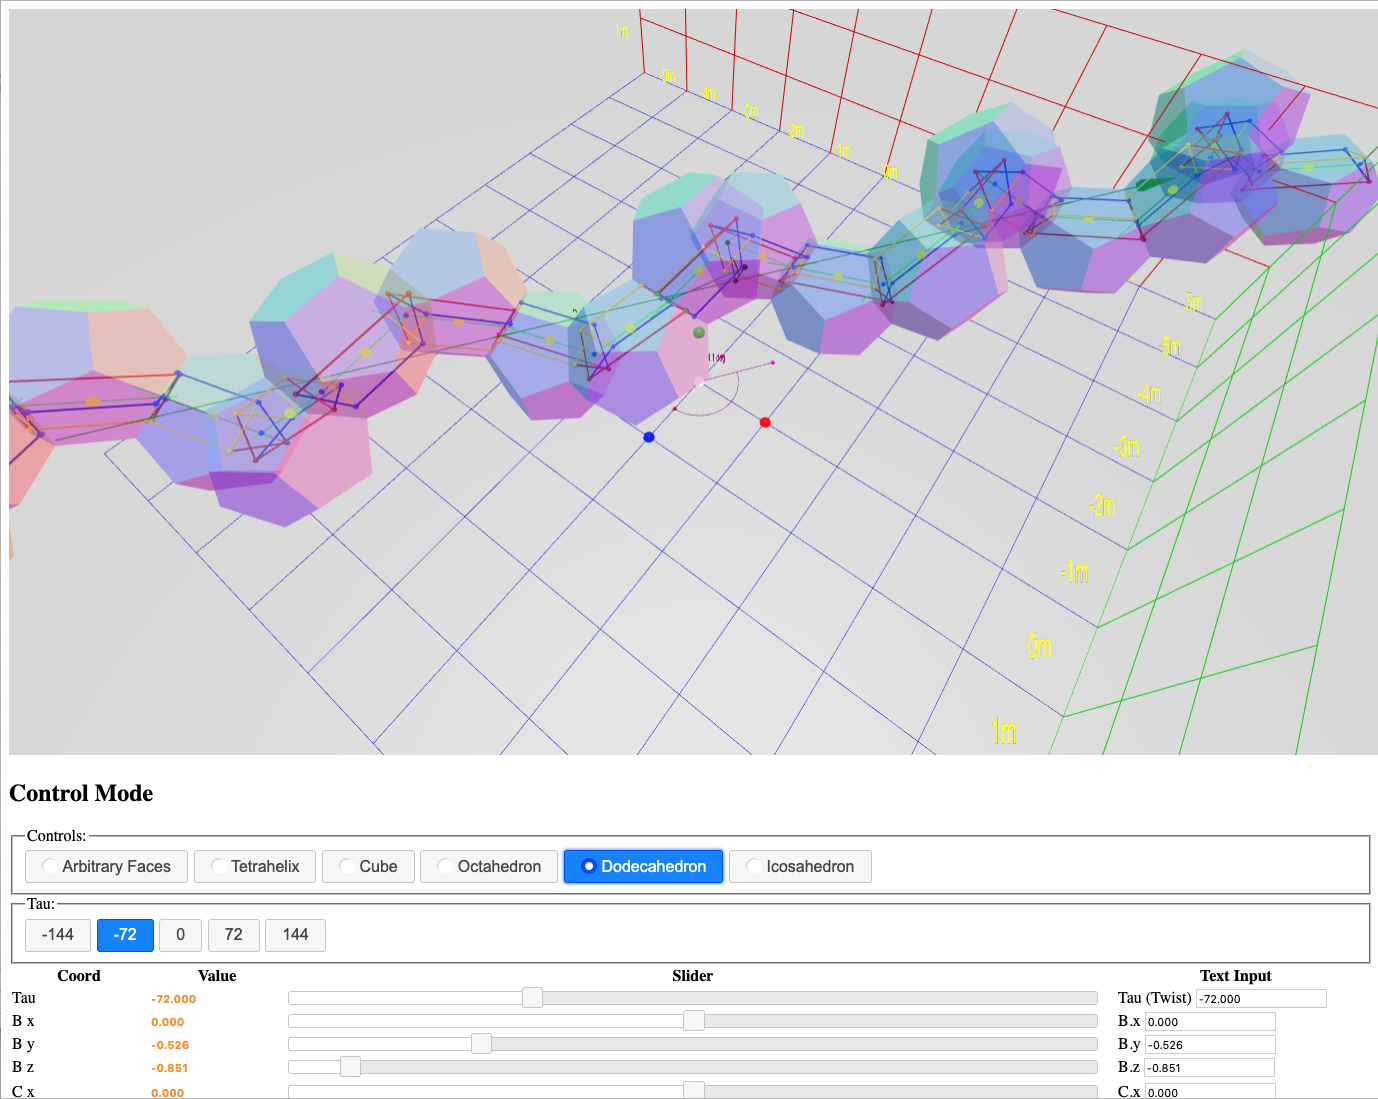
\includegraphics[width=0.80\textwidth]{figures/Dodecahedral.png}
     \caption{Example Segmented Helix Generated From the Dodecahedron}
  \label{fig:dodecahedron}
\end{figure}


\section{A Warm-up: Two Dimensions}

Considering the problem in two dimensions may be a valuable introduction.
Suppose a polygon has two edges, called $A$ and $B$, and length $L$ of the
polygon is defined as the distance between the midpoints of these edges.
Suppose these
polygons are only joined by aligning $A$ of one polygon to $B$ of another polygon, with their midpoints coincident. Further assume that inversions of the polygon are disallowed.  Imagine there exists
countable number of polygons $P_i$ indexed from $0$. Then what shapes can be made by chaining these
polygons together?

\begin{Theorem}
  When polygonal subunits are conjoined with their axes at angle $\theta$, they form a
  circle of radius:
  \[
\frac{L}{2 \sin{\frac{\theta}{2}}}
\]
where if $\theta = 0$ the circle is of infinite radius, that is, a straight line.
  \end{Theorem}
\begin{figure}
     \centering
     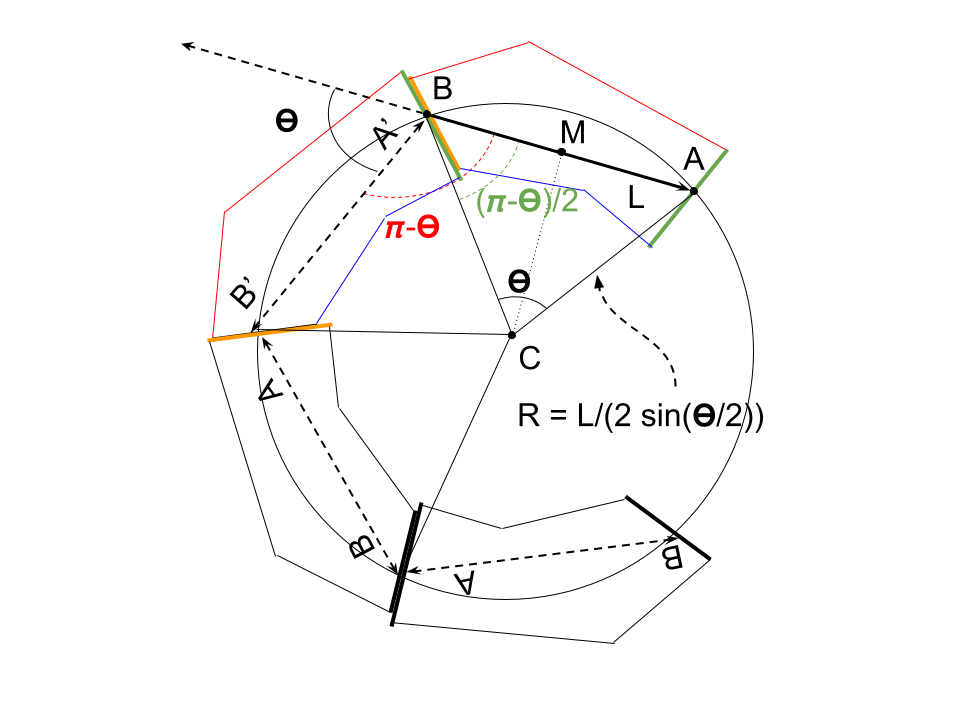
\includegraphics[width=0.80\textwidth]{figures/2DPolygonStacking.png}
     \caption{A 2D analog of a helix generated by repeated subunits}
  \label{fig:prismdiagram}
\end{figure}

\begin{proof}

Each joint $J_i$ between polygons $P_i$ and $P_{i+1}$ will place the axes of the polygons at the same angle, $\theta$, since
these polygons do not change shape. Define $\theta$ to be positive
if we move anti-clockwise from $P_i$ to $P_{i+1}$ and negative if we move clockwise.
If $\theta = 0$, the joints will be collinear.

If $\theta \neq 0$, then form an isosceles triangle $\triangle{ABC}$ in the direction of the second
object, whose axis is $A'B'$.
Form this triangle so that one edge is a bisector of the angle between the axes$\angle ABB'$,
as illustrated in Figure \ref{fig:prismdiagram}.
Make $\angle CAB = \angle CBA$.

Then $\angle ABC = \frac{\pi - \theta}{2}$. Therefore $\angle ACB = \pi - 2(\pi-\theta)/2 = \theta$.
By considering the right triangle formed by midpoint $M$ of $\overline{AB}$ and $C$,
the length of the sides $\overline{AC} = \overline{BC}$ can be computed by the half-angle
of theta:
\[
R = \frac{L}{2 \sin{\frac{\theta}{2}}}
\]
Since the triangles formed by placing a new object are similar and share a side which
is an angle bisector, they all share the point $C$. Therefore, the axis points $A$ and $B$
for each object lies on a circle of radius $R$ with center $C$.
\end{proof}


\label{sec:2d}

\section{The Segmented Helix}

An analogous result holds in three dimensions.

Following the Wikipedia article \cite{wiki:helix},
a helix is set up parametrically:
\begin{align}
    P_x(t) &= r \sin{t}  \\
    P_y(t) &= r \cos{t} \\
   P_z(t) &= b t
\end{align}
Such a helix has a radius of $r$ and slope (if $r \neq 0$) of $b/r$.
The pitch of the helix---the change in $t$ needed to make one complete revolution---is $2\pi b$.
Note that a helix may be degenerate in two ways.
If $r = 0$, these equations become a line. If $b = 0$, these equations describe a circle in the $xy$-plane.
If $r = 0$ and $b = 0$, the figure is a point.

Such helices are continuous, but it is stacks of discrete objects under investigation.
A goal is to derive
the parameters for a continuous helix from such discrete objects by studying
a helix evaluated at integral points. Call such an object a {\em segmented helix}.
A segmented helix may be thought of as function that, given an integer, gives back a point in
3-space.
\begin{align}
    P_x(n) &= r \sin{n \theta}  \\
    P_y(n) &= r \cos{n \theta} \\
   P_z(n) &= n d
\end{align}

$d$ is the distance or {\em travel} along the helix axis between adjacent joints. In this canonical representation the helix axis is
the $z$-axis.
$\theta$ is the rotation around the $z$-axis
between adjacent points.
$r$ is the radius of the segmented helix.
Note that if $\theta = \pi$, a third form of degeneracy (to the human eye) occurs:
that of a segmented helix
which is a zig-zag contained completely within a single plane.

If one thinks of the segmented helix as describing a polyline in 3-space,
the properties of that polyline are of interest.
Considering only the {\em intrinsic} shape of the segmented helix that
are independent of position and orientation in space,
there are three degrees
of freedom: $r,d,$ and $\theta$.

\begin{figure}
     \centering
     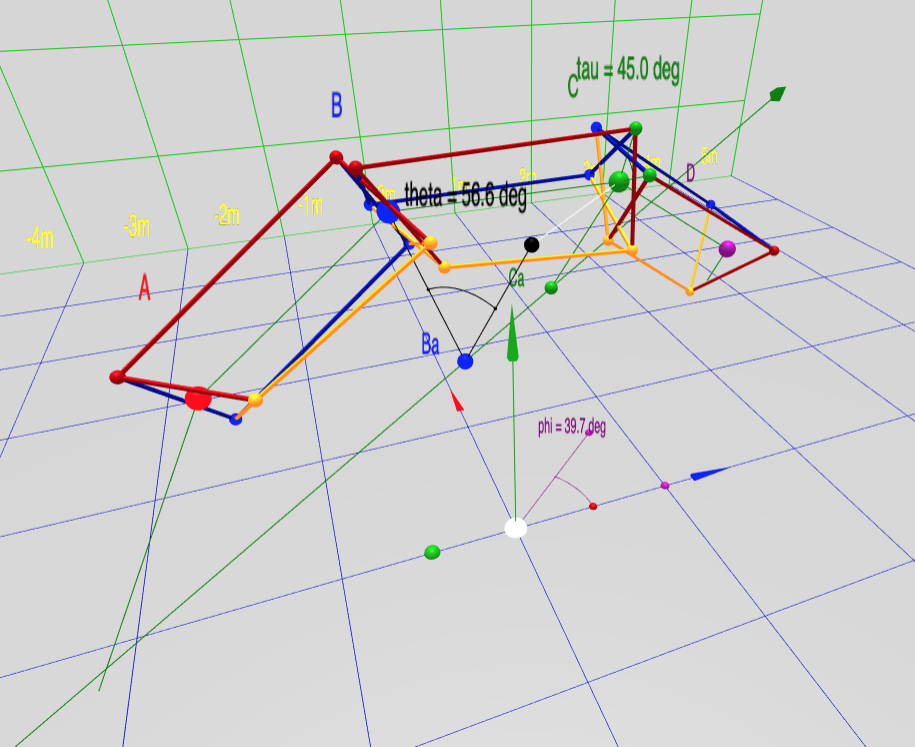
\includegraphics[width=0.80\textwidth]{figures/ABCDFigure.png}
     \caption{Naming of measures}
  \label{fig:naming}
\end{figure}

Figure \ref{fig:naming} demonstrates naming convention concepts.
It is a screen shot taken from the interactive website\cite{segmentedhelixinteractive}.
The software allows parallax by supporting interactive rotation,
which makes the 3D structure easier to perceive;
please visit the interactive page during this discussion of naming conventions.

In Figure \ref{fig:naming} and the website, we represent the object as a prism
with triangular cross-section, because this is
the simplest physically realizable macroscopic object that supports a face-to-face connection.
In this diagram, the
points $A,B,C$, and $D$ are represented by the sphere of the same color as the label. The view is roughly in the direction of
the axis of the segmented helix, which is drawn as a dark green arrow, pointing in the positive $z$ and positive $x$ direction,
parallel to the $XZ$-plane.
For ease of viewing, the entire segmented helix has been raised by two units on the $y$ axis.
The segment $\overline{BC}$ has coordinate $y = 2$, is aligned with the $z$-axis, and centered in the $z$ direction.

The positive $x,y$ and $z$ axes are shown by the red, green, and blue axis arrows, respectively.
Following computer graphics convention, the $y$ axis is oriented vertically.
The points $A,B,C$, and $D$ correspond to $P(0), P(1), P(2)$, and $ P(3)$, respectively,
for a segmented helix aligned
to the raised axis (not the $z$-axis).
A thin green polyline represents the segmented helix, and thus connects the joints $A,B,C$, and $D$.
The points are wrapping around the axis clockwise, with an angle of $\theta = 56.6 \degree$ as
shown by the on-screen protractor as the rotation from one point to the next. As will be explained in Section \ref{sec:facenormal},
$\tau$ is the face-on-face joint rotation, in this case of $45 \degree$.
The helix angle $\phi = 39.7 \degree$ is rendered by a protractor on the $y = 0$ plane;
this is the angle between the axis
and of the helix and the $z$ axis, and therefore the angle of any one segment against the helix axis.

Any point on the segmented helix has a closest point on the axis of the helix.
In particular, the points closest to the
joints are called {\em joint axis points}.
Then $d$ is the distance along the axis between consecutive joint axis points.

A line is drawn from the blue point $B$ to a black sphere on the helix axis,
the joint axis point, denoted $B_a$. Analogously, $C_a$ is the point
on the axis closest to the green point $C$.


A segmented helix located in space is completely determined by
the parameters $r,d,\theta$,
a vector describing the axis
of the helix, and the position of any one joint.

Because the segmented helix is a discrete structure, one can reframe the concept of {\em pitch} as {\em sidedness $s$}:
how many segments (sides)
make a complete rotation?

The following concepts and conventional variable names for them will be related:
\begin{itemize}
\item $L$ is the distance between any two adjacent joints (between $B$ and $C$, for example).
  \item $r$ is the distance between a joint and the helix axis (between $B$ and $B_a$ for example).
  \item $\theta$ is the rotation about the helix axis between two consecutive joints.
  \item $c$ is the length of a chord formed by the projection of the segment between two points projected along the axis of the segmented helix (a chemist may recognize this as the distance between residues on a {\em helical wheel} projection).
  \item $d$ is the distance along the axis of the helix between any two joint axis points (between $B_a$ and $C_a$ in Figure \ref{fig:naming}, for example, rendered as a small black and blue
    sphere, respectively).
\item $\phi$ is the angle between any vector between two adjacent joints and the axis of the helix. In physical screws used in mechanical engineering, this is analogous to the {\em helix angle} \cite{wiki:helixangle}.
  \item $p$ is the pitch of the helix, the distance traveled in one complete rotation.
  \item $s$ is the number of segments in a complete rotation (in general not rational).
\item  Finally, we find it useful to define the {\em tightness} of a segmented helix
as travel divided by radius, a number
analogous to the extension of a coil spring or slinky.
A torus-like segmented helix has zero tightness and a zig-zag has
maximum tightness. The letter $t$ represents tightness.

  \end{itemize}
These quantities are related:
\begin{align}
    c &= 2r\sin{\frac{\theta}{2}} \\
    L^2 &= c^2+d^2  \\
    \arctan{\frac{c}{d}}  &= \phi \\
    s &= \frac{2 \pi}{\theta} \\
    d &= L \cos{\phi} \\
    p &= d \cdot s \\
    t &= d / r
\end{align}

Measuring $\phi$ demands a decision on the sign of the direction of the axis,
which is arbitrary and not based on the
physical shape.

Sections \ref{sec:screws}, \ref{sec:pointaxis} and \ref{sec:facenormal}
relate these properties to properties intrinsic to the joint or interface between
two segments or objects in the segmented helix.

\label{sec:SegmentedHelix}

\subsection{Sign Conventions for Spatially Located Segmented Helices}

When thinking about the overall shape of a segmented helix, one is
likely to be interested in the absolute magnitude of its intrinsic
properties.

However, when doing doing computer graphics work or kinematic
calculations, the sign conventions are critical. Because this
paper wishes to emphasize the continuum of shapes produced by
changing an object used to generate the segmented helix, and,
in particular, is interested in the degenerate helix which
produces toroidal figures, it is preferable to be able to discuss
the axis of a segmented helix as existing even when the
figure has no travel along the axis (that is, when $d = 0$).

Therefore adopt the following conventions:
\begin{itemize}
\item A right-handed coordinate system.
\item The helix axis is a normalized vector
  which never vanishes.
\item The travel along the axis ($d$) is negative when
  the helix is anti-clockwise (that is, when motion from
  joint $n$ to joint $n+1$ appears anti-clockwise when $\theta < \pi$,
  zero when toroidal), and
  positive when the helix is clockwise.
\item $\theta$ is never negative.
\end{itemize}

\section{The Intrinsic Properties of Periodic Chains of Solids}

Although fairly obvious from Chasles' Theorem, in order to prove Observation \ref{obs:lords},
additional clarification is helpful.
If chains of identical repeated 3D units are conjoined identically, they are {\em periodic chains},
and they generate a segmented helix coincident on their joints.
Identical objects conjoined via a rule
produce periodic chains of objects that are uniformly intersected
by segmented helices and may be degenerate in one of
three ways that might not strike the human eye as a helix at first glance:
\begin{enumerate}
\item The segments may form a straight line. (For example, see Figure \ref{fig:pearlshaft}).
\item The segments may be planar about a center, forming a polygon or ring. (For example, see Figure \ref{fig:thewheel}).
\item The segments may form a planar saw-tooth or zig-zag pattern of indefinite extent (For example, see Figure \ref{fig:planarzigzag}).
\end{enumerate}

\begin{figure}
     \centering
     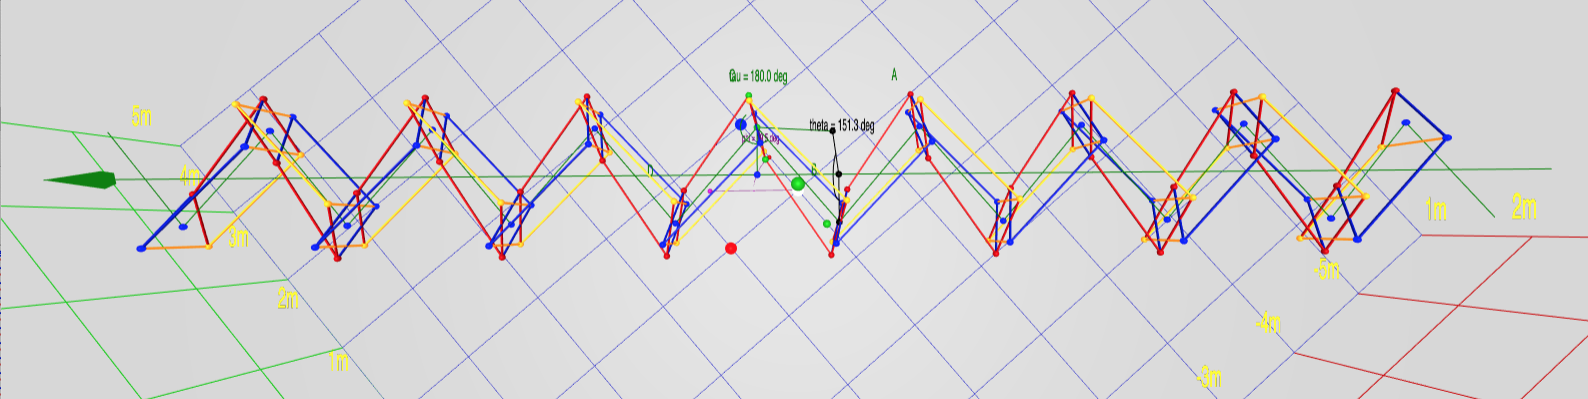
\includegraphics[width=0.80\textwidth]{figures/PlanarZigZag.png}
     \caption{A Planar Zig-Zag}
  \label{fig:planarzigzag}
\end{figure}

There are two complementary ways of learning about such segmented helices.
In one approach, we may have knowledge of the segmented helix and
wish to learn about the subunits and the rule with which the subunits are combined.
For example, we may have microscopic objects such as proteins
or atoms, and we know from crystallography something about the positioning of these objects, without
knowing ahead of time the angles at which these objects would combine in their natural environment.
In this case, we use a variant of a linear algebra method\cite{kahn1989defining}
for determining the radius, travel, and ``twist''
of the segmented helix ({\em twist} will be defined precisely below).

In the other approach, one may know {\it a priori} exactly the
relevant properties of the objects and the rule with which they combine
and seek to compactly describe the segmented helix they create.
For example, a mathematician may consider a chain of dodecahedra,
or a woodworker may cut identical flat-faced chunks of maple wood,
which are to be glued together face-to-face.
In these cases, everything about the objects and the rules for conjoining
is known before the first two objects are glued together.
Call this the {\em joint face normal method}, because
it can be simulated by joining two flat faces together with a specified twist,
even if the objects in question
do not actually have a physical face (such as molecules).

In both cases, it is useful to understand how a change in a face normal
or a twist affects the parameters
of the segmented helix,
and, conversely, useful to be able to choose the construction
of the subunits to achieve a particular segmented helix.

In engineering, sometimes the term {\em special helix}\cite{gu2012research}
is used for helical curves on non-cylindrical surfaces.
This paper use the term {\em helix} only in the
sense of {\em cylindrical helix}.

\section{Periodic Chains Produce Segmented Helices}

A periodic chain is, in fact, a simple object which demonstrates tremendous symmetry.
Before using this symmetry in the construction of the segmented helix corresponding to a periodic chain,
it is valuable to
prove that such a segmented helix indeed exists for every periodic chain.
Because periodic chains are merely a clarification of the ``identical structural subunits''
of Observation \ref{obs:lords},
this theorem proves that observation.

\begin{Theorem}[Segmented Helix]
  \label{thm:helix}
  Consider $N$ identical objects which each have two points, $A$ and $B$, called {\em joints}. Call
  $\overrightarrow{AB}$ the {\em axis} of this object.
  Consider the frame of reference for this object to have
  its axis on the $z$-axis with $B$ in the positive direction, the
  midpoint of the object being at the origin.

  Consider any rule that conjoins $A$ of object $i+1$ to $B$ such that
  from the frame of reference of $i$, the object $i+1$ and anything rigidly
  attached to it is always in the same position in the frame of reference for $i$.
  Informally, $i+1$ ``looks the same'' to $i$, no matter what $i$ is chosen, $i < N$.
  Call a chain of $N$ identical rigid objects conjoined via a rule that
  conjoins $A_{i+1}$ to $B_i$ in such a way that every vector
  of $B$ is always in the same position relative to a frame of reference
  constructed from $A$, a {\em periodic chain.}

  Any periodic chain of three or more objects has a unique segmented helix
  whose segments correspond
  to the axes of these objects.
\end{Theorem}

\begin{proof}
  By induction.

  Base Case ($k = 3$):

  Take an object $A$ with axis $\overrightarrow{AB}$.
  By Chasles' theorem\cite{wiki:chasles}
  there is a screw axis $\overrightarrow{S}$,
  a set of rotations,  and a transposition $d$ which moves
  the first object to the
  position where the second object $B$ with axis $\overrightarrow{BC}$ is.
  Take one of the rotation angles of smallest value.
  Construct the points $A'$, $B'$ and $C'$ as the closest points
  to $A,B$ and $C$ on this screw axis. These points are collinear by construction.

  Now add the object $\overrightarrow{CD}$ to object $\overrightarrow{BC}$
  by the rule of periodic chains. Consider the points
  $B'$ and $C'$ from $A$'s frame of reference. Let $d = \| \overline C' - \overline B' \|$.
  Construct the point $D'$ on the screw axis as the point closest to $D$ on that line.

  Because $\overrightarrow{C'D'}$ in object $B$'s frame or reference must look like $\overrightarrow{B'C'}$ in $A$'s frame of reference,
  the distance $\| \overline D' - \overline C' \| = d$.
  From $A$'s frame of reference, $A'B'C'$ are collinear, so the points $B'C'D'$ must be collinear in
  $B$'s frame of reference.

  In any frame of reference, if $A'B'C'$ are collinear and $B'C'D'$ are collinear, then $A'B'C'D'$
  are collinear.

  Now, looking backward from $\overrightarrow{CD}$ towards $A$, the length $\overrightarrow{A'B'}$ must be the same as the
  length $\overrightarrow{B'C'}$ so as to not violate the rule. So $d = \| \overrightarrow{A'B'} \| = \| \overrightarrow{B'C'} \| = \| \overrightarrow{C'D'}\|$.
  Similarly let $r = \| \overrightarrow{B B'} \|$. Then $r = \| \overrightarrow{C C'} \|$ by construction.
  By the rule of conjoining, the vector $\overrightarrow{A A'}$ is a rigid transformation of
  $\overrightarrow{B B'}$,
so $r = \| \overrightarrow{A A'} \|$.
  By symmetry, $r = \| \overrightarrow{D D'} \|$.
  Compute $\theta$ as the rotation about $\overrightarrow{S}$ that takes $\overrightarrow{B B'}$
  into $\overrightarrow{C C'}$. By the rule
  of attachment, $\theta$ also takes $\overrightarrow{C C'}$ into $\overrightarrow{D D'}$
  and $\overrightarrow{A A'}$ into $\overrightarrow{B B'}$.

  Next, construct a segmented helix, of radius $r$, distance $d$,
  and angle $\theta$. The segmented helix axis and joints can be positioned coincident with the screw axis
  $\overrightarrow{S}$ so
  that $H_0 = A$. Then $H_1=B$, $H_2=C$, and $H_3=D$.

  Therefore, for the base case of three objects, there is a segmented helix whose
  segments coincide with the axes of the objects.


  Inductive Case ($k+1$):

  Assume there is a segmented helix coinciding with the first $k$ objects, and
  consider the frame of reference of the $k$th object. The axis and any
  other rigid property of the $k+1$th object stands in relation to object $k$
  as $k$ stood to $k-1$.

  By the assumption of induction, the $k$th object has an axis coincident to
  a segment
  of a segmented helix. Attach vectors $\overrightarrow{A_{k}A'_{k}}$ and $\overrightarrow{B_{k}B'_{k}}$
  from the
  joints of object $k$ to the corresponding axis joints of the segmented helix perpendicularly. Define these
  vectors in the frame of reference for $k$.

  To the $k-1$th object, the tips of  $\overrightarrow{A_{k}A'_{k}}$ and $\overrightarrow{B_{k}B'_{k}}$ vectors ($A'_{k}$ and $B'_{k}$) define
  a line segment which lies on the axis of the segmented helix $H$, with the
  tip of $B'_{k}$ coincident with the tip of $A'_{k-1}$.

  By the rule of conjoining and by induction, since this is true of the $k-1$th object,
  it is true of the $k$th object. Therefore the tips of the $k+1$th object's attached vectors
  $\overrightarrow{A_{k+1}A'_{k+1}}$ and $\overrightarrow{B_{k+1}B'_{k+1}}$
  form a vector $\overrightarrow{A_{k+1}B'_{k+1}}$ which lies on the axis $H$, extending it
  in the same direction. The joint axis of the $k+1$th object therefore coincides
  with the $k+1$th segment of $H$.

  Therefore, by induction, identical objects conjoined by the same rule always
  coincide with some segmented helix, whose parameters are discoverable.
\end{proof}

In engineering, the term {\em helix angle} refers
to the angle between a line tangent to a continuous helix and
the axis of the helix. In segmented helices, this is the same
as the angle between the
axis of each object in a periodic chain and the axis of the
segmented helix coincident to it.

Consider
objects which are, taken as individuals, highly asymmetric.
For example,
the $B$ face does not have to be the same size as the $A$ face. In fact,
the object itself might be shaped like the letter ``C'', and not completely
enclose the axis. Taking the idea further, the object might be spiky
like a stellated polyhedron or a sea urchin, and still be joined by
joints relatively close to the center of the object. (This paper does not
address the issue of self-collision of the objects,
which would have to be considered if attempting to make a period chain
of sea urchins).

It is perhaps not obvious that building a chain of such objects
produces a segmented helix, and therefore that the helix angle is the
same for each object, but this is a corollary of Theorem \ref{thm:helix}.


\begin{Corollary}[Segment Similarity]
  The helix angle of any object axis in a periodic chain is the same.
  \label{cor:symmetric}
\end{Corollary}

\begin{proof}
  The axes of each object coincide with a segment of a segmented helix.
  A segmented helix is completely symmetric no matter in which direction
  of the axis you look down or at which point on the axis you begin. The angle between each pair of objects
  is exactly the same.
\end{proof}

Corollary \ref{cor:symmetric} will be used in the development of {\em PointAxis} algorithm,
in the computation of segmented helix properties, to justify balancing face normals
to produce an intrinsic out-vector, and to apply the {\em PointAxis} algorithm
without actually assigning objects Cartesian coordinates.

\section{Computing Screws and Segmented Helices from Transformation Matrices}
\label{sec:screws}

The rule for how objects in a periodic chain are joined may be
conveniently captured as a transformation
matrix.
In general, a human engineer will have to compute this transformation matrix from some other
information, such as the face-to-face conjoining rule.
We discuss how to do this from joint-face normal
vectors in Section \ref{sec:facenormal}. However, a transformation matrix clearly
captures the idea of repetition.
Since by definition the objects in the chain are the same shape,
moving one object into a new position and placing an identical copy of that object in that position
are practically the same.

Using standard screw theory\cite{wittenburg2016kinematics,wiki:screwaxis},
a screw can be computed from such
a transformation matrix. This consists of the axis of the screw $\overrightarrow{S}$,
a point on the screw axis $P$,
the rotation $\theta$ around the axis, and the
transposition, or travel, along the axis of one transformation.

Neither a transformation matrix nor its corresponding screw transformation
completely define all of the intrinsic
properties of a segmented helix. In particular, a matrix $\bm{M}$ maps any point $p$ to a point $p'$.
Since this applies to all points no matter how far from the screw axis (axis of rotation), and
such transformations preserve distance to this axis (the radius), the radius of a segmented helix
is not determined by a transformation matrix or a screw. Since the helix angle $\phi$ changes
with radius for a helix of a given pitch, $\phi$ is not determined.

However, given a screw and one point on the axis of the screw fixing it in space
and the location of one joint, all of the properties of the segmented helix are completely determined.

The software behind the interactive website implements the calculation of the screw
directly from a transformation matrix, and
the additional routines which determine all intrinsic properties from a joint position (making
certain arbitrary alignment choices without loss of generality).

Although not original to this paper, it is
difficult to find clear documentation on how to calculate the
screw from the transformation matrix.
We therefore include an exposition here, in hope it will be useful,
and a valuable addition to the code in the source code repository to a programmer seeking to duplicate
this functionality.

\subsection{Computing the Screw Axis from a Transformation Matrix}

The goal is to compute a normalized vector $\hat{\overrightarrow{H}}$ aligned with the screw
axis of the transformation composed and effected by a transformation matrix $\bm{R}$.

In order to be robust, it is valuable to check that the transformation
matrix is a rigid transformation\cite{wiki:rigid},
as Chasles' theorem applies only to rigid transformations.
Transformation matrices in homogeneous coordinates, as typically used in kinematics
and computer graphics, are convenient for this purpose, allowing the transformation
represented by a matrix to be effected by simple multiplication.

The angle of rotation is computable from the trace of $\bm{R}$, $Tr(\bm{R})$.
\begin{align}
  \theta &= \arccos{\frac{Tr(\bm{R}) - 1}{2}}
\end{align}
Technically, $\arccos$ is multi-valued, but take $\theta$
to be in its principle range, $0 \leq \theta \leq \pi$.
If $\theta$ is $0$ or a multiple of $\pi$, then we have the zig-zag
degenerate case; the method of computing $\overrightarrow{H}$ from the rotation
basis of $\bm{R}$ is numerically unstable.
However, in this case
we can compute the direction vector $\overrightarrow{H}$ as the difference vector
between an arbitrary point $q$ (a 4 $\times$ 1 vector in homogeneous coordinates)
and its transformation performed
twice. Informally, this is a ``zig, then a zag''.
\begin{align}
  \overrightarrow{H} &= \bm{R} ( \bm{R}( q)) - q
\end{align}
(Note that in general $\overrightarrow{H}$ is not normalized, $\overrightarrow{H} \neq \hat{\overrightarrow{H}}$.
Also recall that multiplication by a transformation matrix
produces a point that is in a new position representing
the transformation).

In other cases, $\overrightarrow{H}$ can be computed from the direction
cosines of $\bm{R}$\cite{wiki:rotation}:
\begin{align}
  R &=     \begin{bmatrix} a & b & c' & x \\ d' & e & f & y\\ g & h & i & z\\ 0 &  0 & 0 & 1\end{bmatrix} \\
    \overrightarrow{H} &=  \begin{bmatrix} h - f \\ c' - g \\ d' - b \\ 1 \end{bmatrix}
\end{align}
(The variables $c'$ and $d'$ are primed to distinguish them from
the symbols for the chord $c$ and the travel along the axis $d$).
The magnitude of $\norm{\overrightarrow{H}} = 2 \sin{\theta}$, which vanishes
when $\theta$ is $0$ or multiple of $\pi$, hence the need
to treat those cases differently.

\subsection{Combining a single joint with the Matrix}

The vector $\hat{\overrightarrow{H}}$ gives the direction of the
axis of the helix, but does not give a point which fixes
it in space.
Although the matrix $\bm{R}$ in general produces both a rotation
and a translation in space, the distance between $q$ and $\bm{R}q$
in general depends on how far $q$ is from the axis of rotation.
If, however, we are given a single a joint $B$ in addition to
$\bm{R}$, then we can completely determine the entire segmented helix.
$C$ is computed from $\bm{R}$:
\begin{align}
  C &= \bm{R}(B) \\
 \overrightarrow{BC} &= C - B\\
\end{align}
Then $d$ is computable as a projection:
\begin{align}
  d = \overrightarrow{BC} \cdot \hat{\overrightarrow{H}}
\end{align}

These are the only properties that can be computed from the
matrix $\bm{R}$ alone, but given the length $L$ along the
object axis ({\em not} the helix axis) of an object
the helix parameters are computable, based on relations
already given in Section \ref{sec:SegmentedHelix}.

The chord of the segmented helix (that is, length of an object of
axis length $L$
projected along $\overrightarrow{H}$) is:
\begin{align}
  c = \sqrt{L^2 - d^2}
\end{align}
Knowing the chord $c$ and the amount of rotation $\theta$
allows us to compute the radius:
\begin{align}
  r = \frac{c}{2 \sin{\theta}}
\end{align},
unless the chord is $0$, in which case the radius is $0$.
The helix angle $\phi$ is a a function of $c$ and $d$:
\begin{align}
    \phi &= \arctan{\frac{c}{d}}
\end{align}

Sidedness and pitch ($s$ and $p$) follow directly.


\begin{figure}
     \centering
     
\includegraphics[width=0.80\textwidth]{figures/ThreeMemberDiagram.png}
     \caption{Three Symmetric Members}
  \label{fig:threemembersdiagram}
\end{figure}

From these one may produce the joint axis point $B_a$ which is the
point on the helix axis closest to $B$.

Figure \ref{fig:threemembersdiagram}
may be useful in picturing the following quantities.
To do this, conceptually construct the midpoint,
$\overrightarrow{M}$
of $\overrightarrow{BC}$ and utilize the fact that the vector
from $\overrightarrow{M}$ to its closest point on the axis $M_a$ (call this vector $\overrightarrow{Q}$) is perpendicular
to the plane containing both $\overrightarrow{BC}$ and $\overrightarrow{H}$. Therefore,
its direction is constructible via cross product, and
its length $l$ is computable from the radius and chord. $M_a$
is the midpoint of $B_a$ and $C_a$, so just move back
half the travel $d$ along the vector $H$ to get $B_a$.

\begin{align}
  \overrightarrow{M} &= \frac{B + C}{2} \\
  \overrightarrow{Q} &= \overrightarrow{BC} \times \hat{\overrightarrow{H}} \\
  l &= \sqrt{r^2 - \frac{c}{2}^2} \\
  \overrightarrow{Q'} &= -\frac{Q}{l} \\
  B_a &= \overrightarrow{M} + \overrightarrow{Q'} - \frac{d}{2}\hat{\overrightarrow{H}}
\end{align}

Thus, given only the transformation $\bm{R}$, the length $L$, and one
joint $B$, one may compute all of the intrinsic properties
($r,\theta,d,c,\phi$) of
the segmented helix and position it in space via $\overrightarrow{H}$ and $B_a$.

As is common in kinematics\cite{funda1990computational}, there are many ways to represent
the same physical or mathematical situation.
Four consecutive joint positions also completely determine a segmented helix, as presented below.
Because joints can be computed from transformation
matrices and transformation matrices from joints,
which method of calculation is preferable is largely
a matter of choice and clarity.
The code at the interactive website
in fact codes both approaches and compares them as an automated test to ensure
correctness.

A mechanical engineer, roboticist, or computer graphics expert is
likely to find the computation from the
transformation matrix more natural and convenient.
A chemist or crystallographer is more likely to
have learned the position of four points and wish to compute from that.

\section{{\em PointAxis}: Computing Segmented Helices from Joints}
\label{sec:pointaxis}

Kahn\cite{kahn1989defining} has given a method for computing
the axis of a helix in the context of chemistry.
This method uses the observation that the angle bisectors
of the segments on a segmented helix are perpendicular to
and intersect the axis of the helix.
Because chemical helices may not be perfect and because the measurement of positions may not be perfectly accurate,
it is common for chemists to use regression and fitting methods to fit helix parameters to observed positions
on the helix.
Kahn's method was a prelude to some error-tolerant methods applicable to
the realm of organic chemistry\cite{enkhbayar2008helfit}.
This paper is concerned only with pure geometry. Also, Kahn was writing in 1989,
and more convenient computing tools are now available.
The algorithm presented, called {\em PointAxis}, here can be considered a modification of Kahn's algorithm,
which relies on the ability, working in the realm of pure geometry, to position the segments on the axes
to simplify the derivation and computation.

\subsection{A Sketch of the 4-Point Method}

Using tools from linear algebra and well-documented algorithms, a sketch of finding the segmented helix from
four consecutive known points $A,B,C$, and $D$ is:
\begin{itemize}
\item Construct a rigid transformation that places the points conveniently on the $z$-axis and balanced
  around the $y$-axis.
\item Compute the bisectors of the angle between object axes $ \angle{ABC}$, called $\overrightarrow{B_b}$ and the
  bisecting angle $\overrightarrow{C_b}$ of $\angle{BCD}$.
  If the points are collinear, they are a special case.
\item Because these angle bisectors point at the axis of the segmented helix, their cross product is a vector
  in the direction of the axis. If $\overrightarrow{B_b}$ and $\overrightarrow{C_b}$ are parallel or anti-parallel the cross product is not defined
  and we have special cases.
\item  Otherwise the vectors $\overrightarrow{B_b}$ and $\overrightarrow{C_b}$ are skew, and the algorithm for the closest points on
  two skew lines provides two axis points $B_a$ and $C_a$ on these vectors which
  are the closest points on those lines and are also points on the helix axis.
\item The distance between $B_a$ and $B$ is the radius, and the distance between $B_a$ and $C_a$ is the travel $d$ along the axis.
  \item The angle between $\overrightarrow{B - B_a}$ and $\overrightarrow{C - C_a}$ is $\theta$.
\end{itemize}

\subsection{Rotating into Balance from Face Normal Vectors}

\label{sec:balance}



In order to use the {\em PointAxis} algorithm, we need a way
to compute points $A$ and $D$ in balance around the axis $BC$.

\begin{figure}
     \centering
     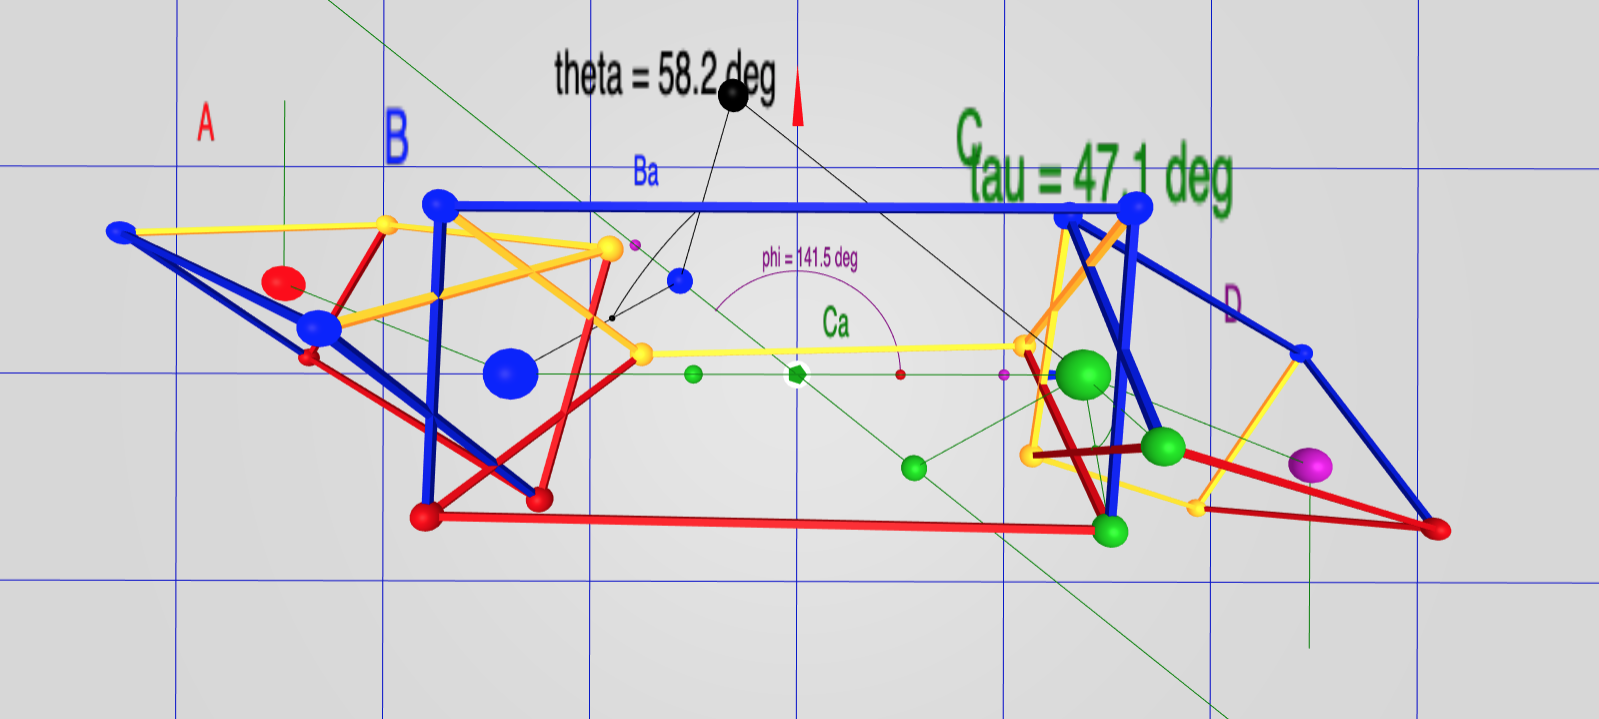
\includegraphics[width=0.80\textwidth]{figures/Balance.png}
     \caption{A Balanced Configuration}
  \label{fig:balancediagram}
\end{figure}


Figure \ref{fig:balancediagram} shows a downward view of a
balanced configuration (though raised above the origin
instead of at the origin).
$A$ (the red sphere) is a reflection of $D$ (the purple sphere) across
the $y$-axis.
Both $A$ and $D$ are hanging downward.
If the structure were hung on a point at the origin, it would
be physically balanced.
As shown in the following, it is always possible to achieve this balance,
even though a single object
itself is not symmetric; in this figure the normal of the $B$ face is not symmetric with $C$ face.

That this is always possible is important enough, if only for
the convenience of calculation, that we consider it a Lemma:
\begin{Lemma}[Balance Lemma]
  For any segmented helix with selected consecutive joints $A,B,C$ and $D$,
  there is a rigid transformation which positions it such that:
  \begin{itemize}
  \item The segment $BC$ is centered on the $z$-axis:
    $(B_x = 0 \wedge B_y = 0 \wedge C_x = 0 \wedge C_y = 0)
    \wedge B_z < 0 \wedge C_z = -B_z$.
  \item The joints $A$ and $D$ are in rotational balance about
    the $y$ axis, as if they were weights hanging downward:
    $A_y = D_y \wedge A_y \leq 0 $ and
    $A_x = -D_x \wedge A_z = -D_z$.
  \end{itemize}
  \label{lem:balance}
\end{Lemma}


% TODO: This should really be labelled a sketch.
%% \begin{proof}

%% A key insight is that Theorem \ref{thm:helix} implies that no matter
%% how lopsided and different
%% the normal vectors  $\overrightarrow{N_B}$ and $\overrightarrow{N_C}$
%% for the joint faces are and no matter what $\tau$ we choose,
%% the relationship of conjoined objects
%% is always the same.
%% After placing $\overrightarrow{BC}$ along
%% the $z$-axis, there is always an angle $\psi$ which will
%% rotate the points $A$ and $D$ into balance (that is, $(A_x = -D_x) \wedge (A_z = -D_z) \wedge (A_y = D_y)$).

%% The key insight to finding $\psi$ is to note that
%% the projections of the $B$ and $C$ face normal vectors
%% projected into the $XY$ plane can be rotated so that they
%% are balanced around the negative $y$ unit vector.
%% Such a projection into the cross-section of the helix is closely related to
%% the {\em helical wheel}\cite{wiki:helicalwheel} plot
%% in the study of alpha helices in proteins.
%% Even if the lengths of the projections of the face normals in $XY$
%% are different, this mechanism works, because by Observation \ref{obs:lords} and Theorem \ref{thm:helix},
%% the points $A$ and $D$ must be symmetric about the segment $\overline{BC}$.

%% By composing this balancing operation with the face-adjoining transformation
%% matrix via {\em adjoinPrism} (see Section \ref{sec:adjoin}), $A$ and $D$ are placed in balance.

%% Note that in the zig-zag case, $A_y = D_y = 0$.

%% \end{proof}


The screw axis may now
be computed from either the four points $A,B,C$, and $D$ or from the transformation
matrix created to balance them.

\subsection{On the Choice of the Screw Axis Direction}

Given only a segmented helix without position in space,
the choice of
direction for the axis is arbitrary.
Changing the decision will make the screw axis point in the negative direction,
change the sign of the travel $d$ along the axis, and change $\phi$ to be $\pi - \phi$.

As can be seen from interactive play with the website\cite{segmentedhelixinteractive},
it is entirely possible for the travel along
the axis of the helix to be $0$. In fact, choosing $\tau \approx 0$
tends to produce toruses, which have no
travel along the axis.

One could choose to represent this be making the unsigned length of the vector
representing the axis be the length of the
travel $d$.
However, this would have the drawback that when $d$ is zero it would be impossible to determine
the axis of revolution of the torus.
Although somewhat arbitrary, we have chosen instead to represent the
axis as a normalized vector of unit length
and to allow the travel to be negative. This has the benefit that
changing $\tau$ through (something close to)
zero smoothly changes $d$. However, it creates the problem that as $\tau$ approaches
(something close to) $\pi$ from different directions the signs of the axes are different.
That is, $\tau \approx \pi$ and $\tau \approx -\pi$ describe exactly
the same shape, but in our calculation
they will have different signs for the axes. The radius, pitch and
absolute value of the travel,
which are intrinsic to the shape, will be the same,
but the axis vector, $\phi$, and the sign of $d$ will be different.

\subsection{The 4-Point Method}

Four consecutive points completely determine at least one segmented helix.
Consider
only the helix that makes the least rotation between these points,
though more rapidly rotating helices will also intersect these points.
The {\em PointAxis} algorithm
takes four such points. Without loss of generality $B$ and $C$
are assumed to be centered on the $z$-axis, and that a
rotation has been performed to balance $A$ and $D$ so that $A_x = -D_x, A_z = -D_z$, and $A_y = D_y$. Thus the input to
{\em PointAxis} in fact has only three degrees of freedom, which determine the three intrinsic properties $r,d,\theta$
which completely define the shape of a segmented helix (but not its location in space).


In the derivations below, we rely on certain facts about
the segmented helix formed by the stack of objects, the first
of which is key:
\begin{itemize}
\item By virtue of Lemma \ref{lem:balance}, without loss of generality, think of any member whose faces
  and twist generate a non-degenerate helix as being ``above'' the
  axis of the helix. Furthermore choose to place the object in
  this figure so that $B_y = C_y$, that is, that the members are symmetric
  about the $z$-axis.
  $A$ and $D$ are ``balanced'' across the $YZ$-plane,
  and $A_x = -D_x$ and $A_y = D_y$.
\item Every joint ($A,B,C$, and $D$) is the same distance $r$ from the axis $H$ of the helix.
\item Every member is in the same angular relation $\phi$ to the axis of the helix.
\item Since every member of a non-degenerate helix cuts across a cylinder around the axis,
  the midpoint of every member is the same distance from the axis
  which is, in general, a little a less than $r$. In particular the midpoint $M$
  whose closest point on the helix axis $m$ is on the $y$-axis and
  $\| \overrightarrow{M_m} \| < \| \overrightarrow{B_b} \|$.
\item The points ($A_a,B_a,C_a,D_a$) on the axis closest to the joints ($A,B,C,D$)
  are equidistant about the axis and centered about the $y$-axis. In
  particular, $\| \overrightarrow{B - B_a} \| = \| \overrightarrow{C - C_a} \|$.
\end{itemize}

From the observations that $\| \overrightarrow{B - B_a} \| = \| \overrightarrow{C - C_a} \|$
it becomes clear that the helix axis is in a plane
parallel to the $XZ$-plane, it intersects the $y$-axis, but in general is
not parallel to the $z$-axis.

Because the angle bisectors of each joint are in general skew, and intersect the
axis perpendicularly, the algorithm
for the closest points on two skew lines finds $B_a$ and $B_c$.

However, a segmented helix has
tremendous symmetry, and the angle bisectors are very far from being two
generally skew lines. In fact, by taking advantage of the fact that the
generating rule for an object chain requires similarity in every joint,
the objects can be arranged as in Figures \ref{fig:naming} and \ref{fig:threemembersdiagram}.

{\em PointAxis} takes a length and a point $D$ known to be in
a specific relation to $B$ and $C$.

This careful arrangement of the axes
allows the computation of $\phi$, the angle between the helical axis
and the $z$ axis. This, in combination with symmetry and the knowledge
that the helical axis is in the $XZ$ plane, supports computing the
points on the axis corresponding to the joints directly from $\phi$.

This algorithm coded below is simple enough that Mathematica\cite{Mathematica} can
actually produce a symbolic closed-form formula for all computed valued
in terms of $L, x, y$, and $z$.
However, these formulae are less comprehensible to the
human eye than this algorithm.
Their existence does open
the possibility that, for example, the derivative representing
the change in $r$ with a change in $D$ could be calculated.

\subsection{Degenerate Cases}

Define the angle bisector vectors:
\begin{align}
  \overrightarrow{B_b} &= B - (A + C)/2 \\
  \overrightarrow{C_b} &= C - (B + D)/2
  \end{align}
The fundamental insight that the axis of the helix $H$ can be
computed by a cross product of the angle bisector
vectors ($\overrightarrow{B_b}$ and $\overrightarrow{C_b}$) applies only
when the angle-bisectors have a non-zero length and when
they are not anti-parallel. When they are of zero length, this is
the degenerate case of a straight line coinciding with all segments.
This occurs only when $A_x = 0 \wedge A_y = 0 \wedge A_z = -3L/2$.
In this case:
\begin{align}
  r &= 0 \\
  \theta &= \text{undefined}\\
  d &= L \\
  \phi &= 0 \\
  \overrightarrow{H} &=  \begin{bmatrix} 0 \\ 0 \\ L  \end{bmatrix} \\
  B_a &= B = \begin{bmatrix} 0 \\ 0 \\ -L/2  \end{bmatrix}
\end{align}
$\overrightarrow{H}$ is the direction vector of the helix axis.
In this case there is insufficient information to define $\theta$,
unless it is through other information. For example, when using
the joint-face normal method which specifies
the twist $\tau$ at the faces, then $\theta = \tau$.

When $\overrightarrow{B_b}$ and $\overrightarrow{C_b}$ are parallel and pointing in opposite directions,
the zig-zag degeneracy occurs. Since
$A$ and $D$ are balanced, this occurs only when $A_y = 0$.
In this case (denoting the $x$ component of the $B_a$ vector as $B_{a[x]}$):
\begin{align}
  B_{a} &= \begin{bmatrix} B_{a[x]} \\ B_{a[y]} \\ B_{a[z]}  \end{bmatrix} \\
  \overrightarrow{H} &=  C - A \\
  d &= (C - B) \times \overrightarrow{H} \\
  r &= \norm{\overrightarrow{B_b}} / 2 \\
  c &= 2 r\\
  \phi &= \atantwo{(H_z,H_x)} - \pi/2 \\
  c &= 0 \\
  \theta &= \pi \\
  B_{a[x]} &= \frac{d\sqrt{1 - (d/L)^2}}{2} \\
  B_{a[y]} &= 0 \\
  B_{a[z]} &= -\frac{d^2}{2L}
\end{align}
(Note: $\atantwo$ is the standard two-argument tangent function employed in software packages).

\subsection{Standard Case}

However, the most general case is simpler and can be worked
out with standard linear algebra operations. In the math below,
which is a direct analog of our coded solution, the tremendous symmetry of the ``balance'' condition
permits the computation to proceed with
using mostly scalar operations. There is some hope that
this would allow closed-form expressions to be produced, perhaps
with the aid of a symbolic computation system such as
Mathematica\cite{Mathematica}. If completed, this would
allow us to give closed-form solution to the intrinsic properties
of all the 28 Platonic helices enumerated in Sec \ref{sec:platonic}.

Once $\overrightarrow{H}$ has been calculated, the signed travel along the axis $d$ is
the scalar projection of a segment $\overrightarrow{C - B}$ onto $\overrightarrow{H}$.
From this $\phi$ is directly calculable. $\phi$ allows
a direct calculation of the $x,y$ and $z$ components of the
point $B_a$ on the axis pointed to by $\overrightarrow{B_b}$.
$r$ is the distance between $B_a$ and $B$. $c$ and $\theta$
are easily computed from these values.

\begin{align}
  \overrightarrow{H} &=  \begin{bmatrix} -2 B_{b[y]} B_{b[z]} \\ 0 \\ 2 B_{b[y]} B_{b[x]}  \end{bmatrix} \\
  d &= \frac{L B_{b[x]}}{\sqrt{B_{b[x]}^2 + B_{b[z]}^2}}  \\
  \phi &= \atantwo{(H_z,H_x)} - \pi/2  \\
  c &= \sqrt{L^2 - d^2}
\end{align}

In this approach to calculation, it is easiest
to compute the axis point $B_a$ corresponding to $B$ and
use it to complete our computations.

From trigonometry and utilizing the facts that
\begin{align}
\phi &= \arccos{(d/L)} \\
\sin{(\arccos{x})} &= \sqrt{1 - x^2}
\end{align}
  it
can be shown that
the $x$ and $z$ component of $B_a$ are:
\begin{align}
  B_{a[x]} &= \frac{d\sqrt{1 - (d/L)^2}}{2} \\
  B_{a[z]} &= -\frac{d^2}{2L}
\end{align}

However, this computation exposes another special case: when the
helix angle $\phi$ is $\pi /2$, the segmented helix is
torus-like. In this case the axis point $B_a$ is in fact
on the $y$-axis, and so only $B_{a[y]}$ is need:
\begin{align}
  B_{a[y]} &=  \frac{L B_{b[y]}}{2 B_{b[z]}}
\end{align}
Except for in the toroidal case,  $B_{b[x]}$ must be taken into
account, but it is non-zero, so we can divide by it.
By imagining a plane pressed downward from the
object axis to the helix axis, it is apparent that $B_{a[y]}$
is proportional to a ratio of the angle bisector
$B_{b[y]}/B_{b[x]}$ times the $B_{a[x]}$ value:
\begin{align}
  B_{a[y]} &=  \frac{ B_{b[y]} B_{a[x]}}{ B_{b[x]}}
\end{align}

Having computed all of $B_a$, the remaining intrinsic properties are easily
calculated:

\begin{align}
  r &= \norm{B - B_a}  \\
  \theta &= 2 \arcsin{\frac{c}{2r}}
\end{align}


\subsection{The 4-Point Test}

It is useful to have a test of whether or not four proposed points really do lie on a segmented helix, to see
if they allow valid inputs to {\em PointAxis} algorithm to be computed via rigid
transformation to the $z$-axis.

\begin{Theorem}[Segmented Helix Test]
  Four arbitrary sequential points $A,B,C,D$ are consecutive joints of a segmented helix if and only if
  the segments $\overline{AB},\overline{BC}$, and $\overline{CD}$ are equal length and the scalar projection
  of $\overrightarrow{CD}$ onto $\overrightarrow{BC}$ is equal to the scalar projection of $\overrightarrow{AB}$
  onto $\overrightarrow{BC}$.
\end{Theorem}

\begin{proof}
  ``If'' Case (points on helix imply scalar projections are negations of each other):

  If $A,B,C,D$ are consecutive joints on a segmented helix, then the angle $\eta$ between any two consecutive segments is the
  same. Then:
  \begin{alignat*}{2}
    \norm{\overrightarrow{AB}} &= \norm{\overrightarrow{CD}} &\quad &\text{Given}\\
    \norm{\overrightarrow{AB}}\cos{\eta} &= \norm{\overrightarrow{CD}}\cos{\eta} &\quad &\text{$\eta$ the same for each joint} \\
    \overrightarrow{AB} \cdot \hat{\overrightarrow{BC}} &= \overrightarrow{CD} \cdot \hat{\overrightarrow{BC}} &\quad &\text{def. of scalar projection} \\
  \end{alignat*}

  ``only if'' Case (equal scalar projections and length imply coincident segmented helix):

  If the scalar projections and the lengths are equal, then the cosines of the angles between segments are equal.
  In the range $0$ to $\pi$,
  $\cos{\theta} = \cos{\phi}$ implies $\theta = \phi$. Therefore the angles between the segments are equal.

  By the previous argument of correctness for the {\em PointAxis} algorithm, a rigid transformation always exists
  which balances three such segments. Therefore there always exists a helix axis that
  is in the $xz$ plane that intersects the $y$ axis and is the same distance from $A$, $B$, $C$ and $D$.
  This axis is the axis of a segmented helix which rotates each point similarly, provides the same translation along the axis,
  and maintains the same radius. Hence a segmented helix exists whose joints are $A$, $B$, $C$, and $D$.
\end{proof}

In a single sentence, if the angles (easily measured by scalar projections) and lengths are the same,
they can be brought into our conventional balanced configuration,
and from that configuration it is clear there exists a segmented helix that coincides with all joints.

\subsection{Comparison}

There is one reason one might prefer the transformation matrix method or the point method over the other: with modern
computer algebra systems such as Mathematica\cite{Mathematica} it might be possible to use these ``algorithms'' to produce closed-form
expressions of closed-form (algebraic) inputs. For example, the Platonic solids all have lengths and face normals which
can be specified exactly in closed (though irrational) form.
Thus in the future it might be possible to produce an expression for the
radius of one of the Platonic Dodecahelices of unit edge length.


\section{The Joint Face Normal Method}
\label{sec:facenormal}

{\em PointAxis} takes a point $A$ known to be in a specific, balanced relation
to $B, C$ and $D$. A chemist might know four such points from crystallography
and be able to move them into this symmetric position along the $z$-axis.

However, one might instead know something of the subunits and
how they are conjoined, without actually knowing where points $A$
and $D$ are.

Take as given these intrinsic properties of an object, and additionally the
rule for how objects are laid face-to-face. That is, knowing the length between two
joint points and a vector normal to the faces of the two joints, we almost have
enough to determine the unique stacking of objects. The final piece
needed is
the {\em twist}. When face $A$ of a second objects is placed on face $B$
of a first object so that they are flush (that is, their normals are in opposite directions),
it remains the case that the second object can be rotated about the normals. To
define the joining rule, attach an {\em up vector} to each object, or more appropriately
since we are dealing with a helix, an {\em out vector} that points away from the axis.
Then a joining
rule is ``place the second object against the first, joint point coincident to joint point,
and twist it so that its out vector differs by $\tau$ degrees from the out vector of the first
object.'' In this definition, the out vectors are considered to be measured against the plane
containing the two axes meeting in a joint.

Define the {\em joint plane} to be the plane which contains the two faces meeting in a joint.
Define the {\em joint line} to be the line through the joint perpendicular to the joint plane.
Define the {\em joint angle} to be the angle of the first axis to the second measured about
the joint line.
The twist $\tau$ is the change in the a vector attached to the object rotated about the joint
line by the joint angle. That is, take any vector attached to the first object, place it at
the joint, rotate it about the joint line via the joint angle. $\tau$ is the difference
between the angle of this vector measured against the joint plane and the angle of the
out vector of the second object measured against the joint plane.

If the objects are macroscopic objects which have faces, this is the same as the rotation
of the axis of the second object relative to the first in the plane of the coincident faces.
Define intrinsic properties:

\begin{itemize}
\item Given an object with two identified faces, labeled $B$ and $C$, assume there are normalized
  vectors $\overrightarrow{N_B}$ and $\overrightarrow{N_C}$
  from each of these points that are aligned with the axis of the conjoined object attached to
  that face. These normals might be enforced by the fact that flat faces are joined in the joint plane.
  However, molecules don't have faces; this conjoining relationship may be enforced some other way.
\item The length $L$ of an object, measured from joint point $A$ to joint point $B$.
\item A joint twist $\tau$ defining the change in computed out-vector between objects,
  measured at the joint face.
\end{itemize}

\subsection{Adjoining Prisms with Linear Algebra, Producing a Transformation Matrix}
\label{sec:adjoin}

For computer programmers with a graphics library supporting transformation matrices such
as THREE.js\cite{dirksen2013learning},
it is relatively easy to code the math to adjoin objects
face-to-face based on the face normals, simulating the physical act of
matching flat faces between macroscopic objects.
\begin{enumerate}
  \item Create the transformation the aligns and centers $\overrightarrow{BC}$ on the $z$-axis.
\item Create a translation of $B$ to $C$.
\item Create a rotation of the $z$-axis to  $\overrightarrow{N_B}$.
\item Create a rotation of of $-\overrightarrow{N_C}$ about $\overrightarrow{N_B}$.
  \item Create a rotation of $\tau$ around that axis.
\end{enumerate}
Composing these transformation matrices via multiplication creates a
transformation matrix which takes $B$ to $C$ and $C$ to $D$.

\subsection{Completing the Face Normal Computation}
Assume this functionality
is coded in a subroutine called {\em adjoinPrism} which does this, taking a prism
(including the face normals $\overrightarrow{N_B}$ and $\overrightarrow{N_C}$) and $\tau$
(the rotation inside the plane of the joint) and produces a prism
in a face-to-face position. A byproduct
of balancing the points is a transformation matrix
that takes $C$ into $D$. Having done this, the screw axis is computable,
and hence all of the segmented helix properties,
from either the transformation matrix or the four points.
The code published at the website does both and compares the result as a test.

\section{Changing $\tau$ Smoothly Changes Tightness}

Upon implementing our interactive ability to vary $\tau$, the following
theorem becomes visually apparent.

\begin{Theorem}[Twist Spectrum]
  For any choice of non-parallel face normals having non-zero $x$ or $y$ components,
  changing the twist angle $\tau$ through a complete rotation ($0 \leq \tau \leq 2\pi$)
  smoothly varies the segmented helix
  between a torus and flat cases.
  \label{thm:twistspectrum}
\end{Theorem}




\begin{figure}
     \centering
     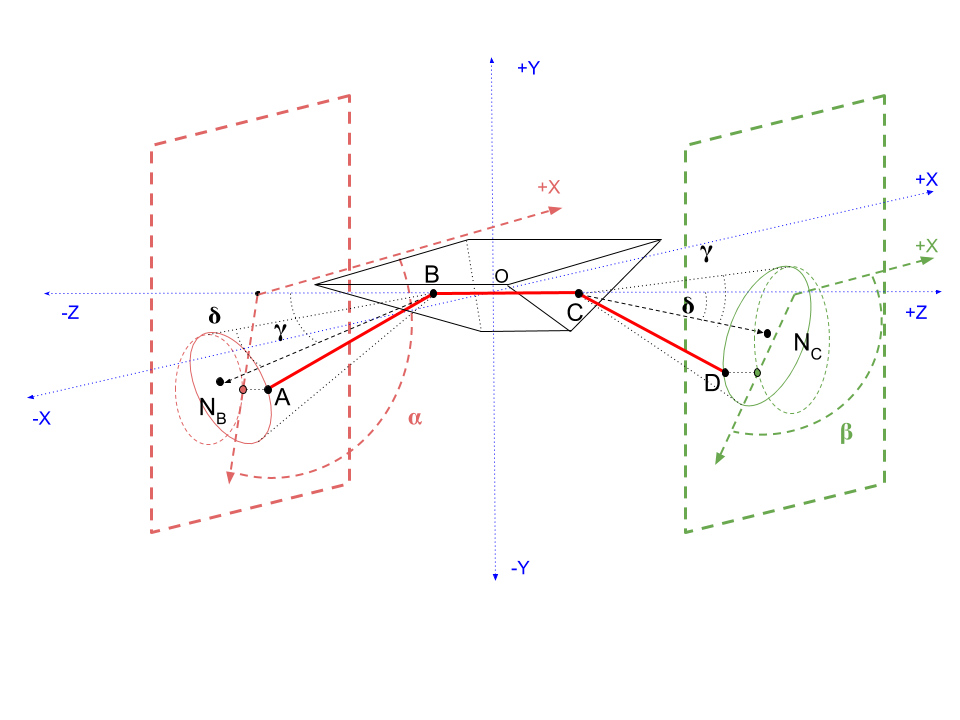
\includegraphics[width=0.80\textwidth]{figures/TwistSpectrumGeneral.png}
     \caption{Twist Spectrum Proof Diagram}
  \label{fig:twistspectrum}
\end{figure}

\begin{proof}
  Figure \ref{fig:twistspectrum} renders an arbitrary
  prism in balanced position. The $B$ joint is on the backside of the
  prism. As usual, $\tau$ is measured against the
  face. The face normals are labeled $\overrightarrow{N_B}$ and $\overrightarrow{N_C}$.
  They are drawn
  to projection planes orthogonal to the object axis, which is $z$-axis
  aligned as per our usual convention. The $\overrightarrow{N_B}$ face normal forms
  an angle $\delta$ with negative $z$-axis, and the $\overrightarrow{N_C}$ face normal
  an angle $\gamma$ with the positive $z$-axis.

  Let the function $\alpha(\tau)$ be the angle formed by the
  projection of the vector $A$ and the origin with the $X$ axis in the $XY$-plane.
  Let $\beta(\tau)$ be the angle of the $D$ projection. $\alpha(\tau)$
  and $\beta(\tau)$ are periodic on $\tau$ ranging between $0$ and
  $2\pi$.

    Let $\gamma$ and $\delta$ be the angle between the $A$ face-vector and
    $B$ face-vectors respectively formed with the
    $\overrightarrow{BA}$ vector and $\overrightarrow{AB}$ respectively.

    If $\gamma \neq \delta$, then one is greater than the other.
    Without loss of generality, assume $\gamma > \delta$.
    Then $D$ moves in a cone
    about the $\overrightarrow{N_c}$ face normal as $\tau$ is varied. The
    angle of the projection of $D$ is $\beta$, which varies as $\tau$
    varies.
    The projection of both $A$ and $D$ move in circles
    potentially tilted to the $z$-axis, thereby
    forming ellipse-like figures in the projection planes.

    By assumption, because $\gamma > \delta$, the
    ellipse formed by $D$ as $\tau$ changes
    strictly contains the origin of the projection plane.
    Therefore, at least one of $\beta(\tau)$  has a range
    containing both $0$ and $2\pi$, since the angle swept out by
    a point on the edge of this figure goes completely around the origin.
    Without loss of generality, let $\alpha$ have that property.

    Both $\alpha$ and $\beta$ are continuous, by the continuity of
    physical mechanisms and the composition of continuous functions.

    Note that although the motion need not be proportional, the sign
    of the motion of $\alpha(\tau)$ is the opposite of the sign of the
    motion of $\beta(\tau)$ as $\tau$ is varied.

    Because $\alpha$ varies between $0$ and $2\pi$ (although
    $\beta$ may not), and because $\beta$ moves in the opposite direction,
    by the Intermediate Value Theorem, there is a $\tau$ where
    $\alpha(\tau) = \beta(\tau)$. Such a point produces a toroid-like
    figure (zero tightness).

    Since $\alpha$ can be moved in a complete circle (between 0 and
    $2\pi$), there is always
    exactly one
    $\tau$ which places $\alpha$ opposite $\beta$
    (i.e., $\alpha = \pi + \beta$). This is the flat case, which
    is the maximal extent of the segmented helix (that is, maximum tightness).

    Now consider the case that $\gamma = \delta$, as illustrated
    in Figure \ref{fig:twistspectrumequal}.

    \begin{figure}
     \centering
     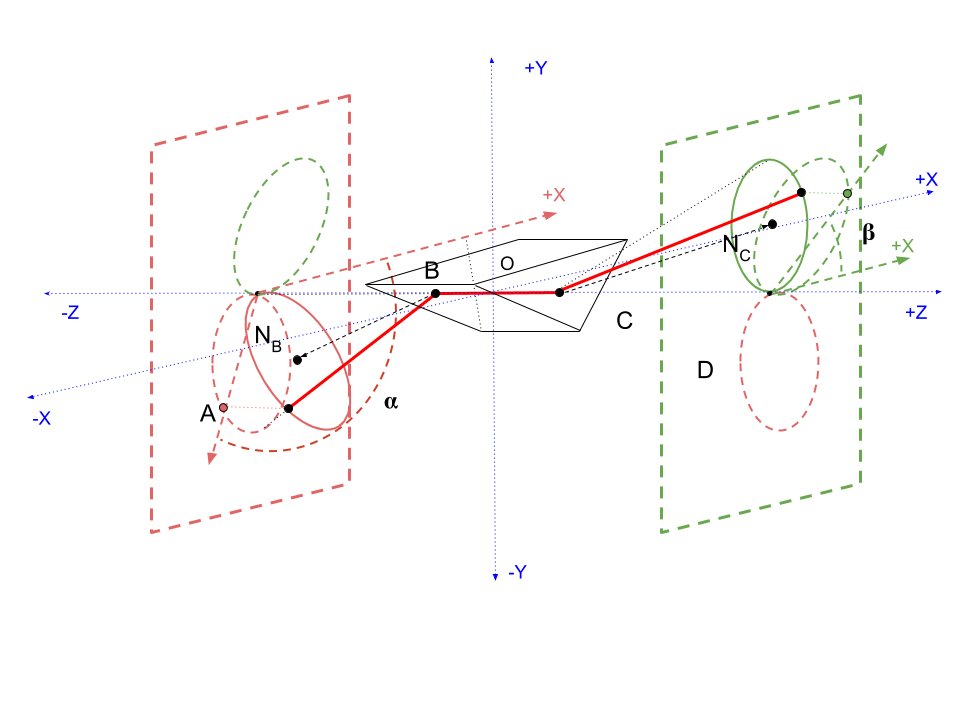
\includegraphics[width=0.80\textwidth]{figures/TwistSpectrumEqual.png}
     \caption{Equal face angle magnitudes}
  \label{fig:twistspectrumequal}
    \end{figure}

    In this case, the edges of the ellipses formed in the projection plane of both $A$ and $D$
    intersect
    the $z$-axis, because there is always a $\tau$ that rotates
    the face about the face normal so that they cancel completely. By our
    proof of segmented helices, this must occur at the same time on both sides,
    because the angle of the $CD$ member with $BC$ must equal the angle of the $AB$ member
    with $BC$.

    Note that the projected ellipses may occur in any relation to each other.
    Figure \ref{fig:twistspectrumequal} illustrates one circumstance in which the face normal
    vectors are pointing in approximately opposite directions.
    If the
    projections of the
    face normals are anti-parallel, they will be exactly opposite each other. In this
    case, the green (D) and red (A) projections will coincide at only one point; this
    is a straight line of a degenerate torus.
        \begin{figure}
     \centering
     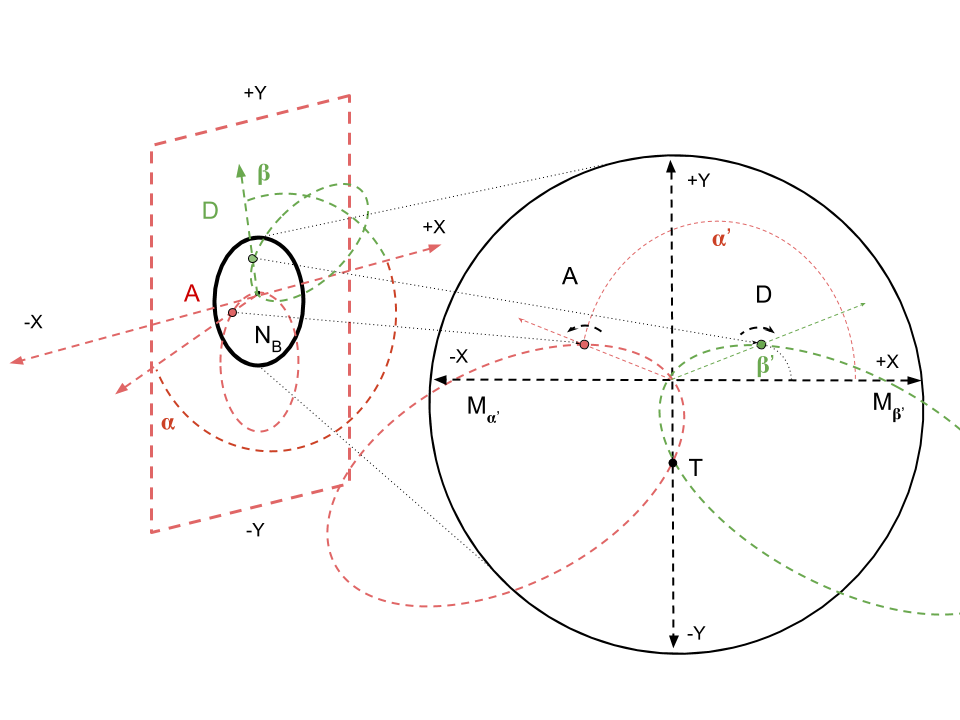
\includegraphics[width=0.80\textwidth]{figures/TwistSpectrumProjection.png}
     \caption{Balanced Projection}
  \label{fig:twistspectrumprojection}
    \end{figure}

    In an unbalanced position, the rate of change of $\alpha(\tau)$ and $\beta(\tau)$
    need not be proportional.
    However, if the entire figure is rotated into
    the conventional balanced configuration for any given $\tau$, then the rate of
    change of $\alpha$ will be exactly opposite $\beta$,
    as illustrated in Figure \ref{fig:twistspectrumprojection}. Let $\alpha'(\tau)$ and $\beta'(\tau)$ be the angles
    formed with the negative $y$-axis in the balanced configuration. By definition of balance about the $y$-axis,
    $\alpha'(\tau) = -\beta'(\tau)$

    This means the
    intersection point of the two projected ellipses (which may be very close to the
    $z$-axis), will always be reached at exactly time ($\tau$): $\alpha'(\tau) = 0 - \beta'(\tau)$.
    This intersection point
    in the balanced configuration is straight down; it is the point at which the projections
    are in the same plane (the plane of the $z$-axis), and at this point the segmented
    helix is a toroid-like figure. Since there is always such an intersection point
    and  $\tau$ can be moved through a full rotation, such a toroidal point can always be reached.
    If the face normals are precisely anti-parallel, this point will occur at the origin,
    and in that case will be a straight line, which is in a sense a degenerate torus-like figure.

    Similarly, the objects can always be twisted to a point where $A$ and $D$ are pointing opposite each other
    as measured from the origin of the projection plane, so that
    $\beta'(\tau) = \alpha'(\tau) + \pm \pi$.
    This is always the ``flat'' or maximally
    extended point of maximum tightness.
    In the balanced convention, this occurs when the projection points are
    coincident with the $x$-axis in the projection plane, as shown in Figure \ref{fig:twistspectrumprojection}.
    Because in this case $\gamma = \delta$ the A and D points are always (even in the first case of this proof)
    at equal angles to the $z$-axis aligned object axis $BC$, the $A$ and $D$ projection points move
    at the same speed (with respect to $\tau$), and they meet the $x$-axis at the same $\tau$ value.

    Thus, when the absolute value of the face normals formed with the $z$-axis are equal,
    the objects can be smoothly twisted through a spectrum between the toroid-like
    figure (zero travel, or $d = 0$, and therefore minimum tightness), and the position of maximal travel.

\end{proof}


It would be more useful and elegant to have a formula for the twist $\tau$ that produces
a torus as a function of the joint face normals, which is future work.
Nonetheless, in the calculator page
the $\tau$ that produces the minimum tightness (torus-like) and maximum tightness (zig-zag) to the
nearest 360-degree is numerically calculated,
with the labels {\em Minimum Tightness $\tau$} and {\em Maximum Tightness $\tau$}.

\section{Checks and Explorations}

\subsection{Qualitative Observations}

When the joint face normals are coplanar vectors, then the minimum tightness $\tau$ is
always $0$, and the maximum tightness occurs when $\tau = \pm \pi$.
These values deviate from $0$ and $\pi$ roughly in proportion
to the non-coplanarity of the normals.

Varying $\tau$ smoothly varies the tightness of the coiling of the helix,
moving through very linear cases towards a torus,
to a torus, to a very linear case on the other side.

In fact it is possible that there is always a ``tightest coil''
which does not self-intersect. If we had many objects,
they could be packed into a convenient space by computing the $\tau$
of the tightest non-self-intersecting coil and stacking them this way.
If $\tau$ can be changed, perhaps via motors in a robot arm,
the object stack smoothly telescopes and contracts forming a
linear actuator.
A repeated molecular subunit that changed shape in
response to an external magnetic or electric field or chemicals in the surrounding
environment would be a telescoping nanomachine or nanoactuator.


\subsection{A Brute-force Approach to Finding Helix Angle from Twist}

The calculation methods described in this paper hardly warrant the name ``algorithm'' when considered from the view of computational complexity;
they are all constant time (for a given fixed precision).
Although involving trigonometric functions, they demand no iteration.

This makes it practical to solve some problems by brute-force iteration.
An example already calculated is the twist $\tau$ which makes
an object product a toroid-like segmented helix, or on the other hand
the $\tau$ value that maximizes linear extent and tightness.
Future work may allow analytic formulae for $\tau$ as a function of
tightness to be developed; in the meantime it is easy enough
to simply evaluate objects at many different $\tau$ values to find a
desired helix angle $\phi$, such as $0$.
Standard numerical optimization can of course be brought to bear, because an objective function
that depends on the parameters of the segmented helix can
be efficiently computed in constant time.

\section{Implications}

One of the implications of having an easily-calculable understanding of the math
is that it may be possible to design helices
of any radius and pitch by designing periodic (possibly irregular) objects.
Combined with slight
irregularities, this means there exists a basis to design molecular helices
out of ``atoms'' which correspond to our objects.

This means that if a structural engineer that wanted to construct a structure exactly 10 meters high
out of a number of repeated objects cast from concrete with an axis length of  exactly $\sqrt{2}$ meters,
they would be able to design the conjoining rule easily.

A modular robot constructed out of repetitions of the same shape-changing module will always
produce a helix
whose precise shape can be controlled by uniformly changing the shape of all of the modules.

\section{Applying to The Boerdijk-Coxeter Tetrahelix}

\begin{figure}
     \centering
     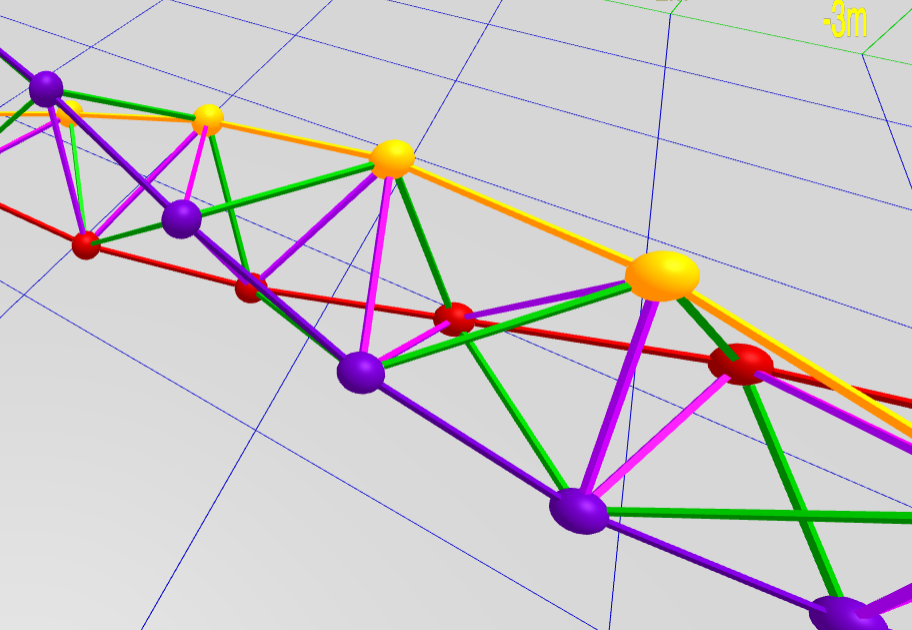
\includegraphics[width=0.80\textwidth]{figures/BCHelixCloseUp.png}
     \caption{Boerdijk-Coxeter Tetrahelix}
  \label{fig:bchelix}
\end{figure}

The Boerdijk-Coxeter tetrahelix (BC helix) (see Figure \ref{fig:bchelix}) is a periodic chain of conjoined regular tetrahedra
which has been much studied\cite{coxeter1985simplicial,sadler2019periodic,fuller1982synergetics,read2018transforming}
and happens to have irrational measures, making it an ideal
test case for these algorithms. Because the face-normals can be calculated and the
positions of the elements of the BC helix directly calculated, we can use
it to test the algorithms, and in fact these algorithms give the same rotation.


\begin{figure}
     \centering
     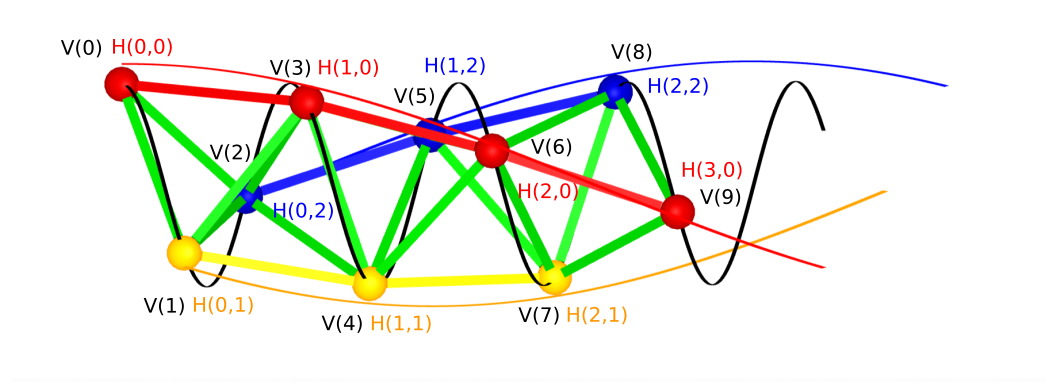
\includegraphics[width=0.80\textwidth]{figures/UnifiedDrawing.png}
     \caption{Node (Coxeter) helix (in black) and rail helices (in red, blue, and yellow),
       different than joint helices}
  \label{fig:helixnodes}
\end{figure}

However, it should be cautioned that the helix which Coxeter identified\cite{coxeter1985simplicial}
goes through every node of every tetrahedron. Constructing the helix going
through only ``rail'' nodes allows irregular tetrahelices to be designed\cite{read2018transforming}
(see Figure \ref{fig:helixnodes}).
However, the segmented helices defined in this paper do neither; rather, it is most natural to
imagine them moving through the centroid of a face of a tetrahedron.
This is a segmented helix of
very small radius ($0.0943$) compared to the other two approaches
($\frac{3\sqrt{3}}{10} \approx 0.5196$) which measure the radius to the
vertex of the tetrahedron, but it has
the advantage that it is far more general. For example, it is
clearly defined if one used truncated tetrahedra.
The rotation of a
segment matches the BC helix analytical solution
($\theta = \arctan{-3/2} \approx 131.810$) (see first line of Table \ref{table:platonic}),
because a screw transformation does not depend on selecting a point for the radius.

In light of Observation \ref{obs:lords} and the segmented helix algorithms, it is possible to
consider the BC Helix and a variety of other segmented helices generated by
face-to-face stacking of Platonic solids, examples called {\em Platonic segmented helices}.

Note this also makes clear that in these cases it is necessary to also specify the {\em twist},
even if perfect face-to-face matching is required.
Thinking of it this
way, there are actually three tetrahedral segmented helices,
depending on which twist modulo 120$\degree$
is chosen (keeping the faces matching): the clockwise BC Helix, the anti-clockwise BC Helix, and the
not-quite-closed tetrahedral torus, similar in appearance to but not quite the same as
{\em toroidal polyhedral}\cite{wiki:toroidalpolyhedra}.
(Five tetrahedra famously lack $\approx 7.356$ degrees of being a perfect toroidal polyhedron
as can be seen from the website which computes $\theta = 70.5288$ for this case,
so the gap is $360 - 5 \cdot \theta \approx 7.356$.)

In the case of the icosahedron, there are in fact many possibilities,
as one need not choose the precisely opposite face as the joining face, and
up to three twists may be chosen.


\section{Confirming Periodic Twists}

The Boerdijk-Coxeter tetrahelix has an irrational rotation about the angle,
meaning that is aperiodic.
There is no number of perfectly regular tetrahedra that can be joined to get back to exactly
the same position.
A recent paper by Sadler, Fang, Clawon and Irwin\cite{sadler2019periodic} has explored this
and given an explicit formula for a {\em twist} exactly as defined in this
paper in order to produce a periodic tetrahelix.

Their formula for period $p$ is:
\begin{align}
  \beta =& 2 \arccos{\frac{\cos{\frac{p\pi}{m}}}{\cos{\varphi}}}
\end{align}
where $\beta$ would be the twist $\tau$ and $\varphi = \arccos{\sqrt{\frac{2}{3}}}$,
the dihedral half-angle of the regular tetrahedron, and $m$ is chosen to
satisfy $\frac{1}{5} \lessapprox \frac{p}{m} \lessapprox \frac{4}{5}$.
Seeking a period of 7, we choose $m = 2$ to satisfy this condition, and
obtain $\approx 80.43 \degree$. It is gratifying that this angle does
in fact produce a period-7 tetrahelix as shown in Figure \ref{fig:periodseven}.

\begin{figure}
     \centering
     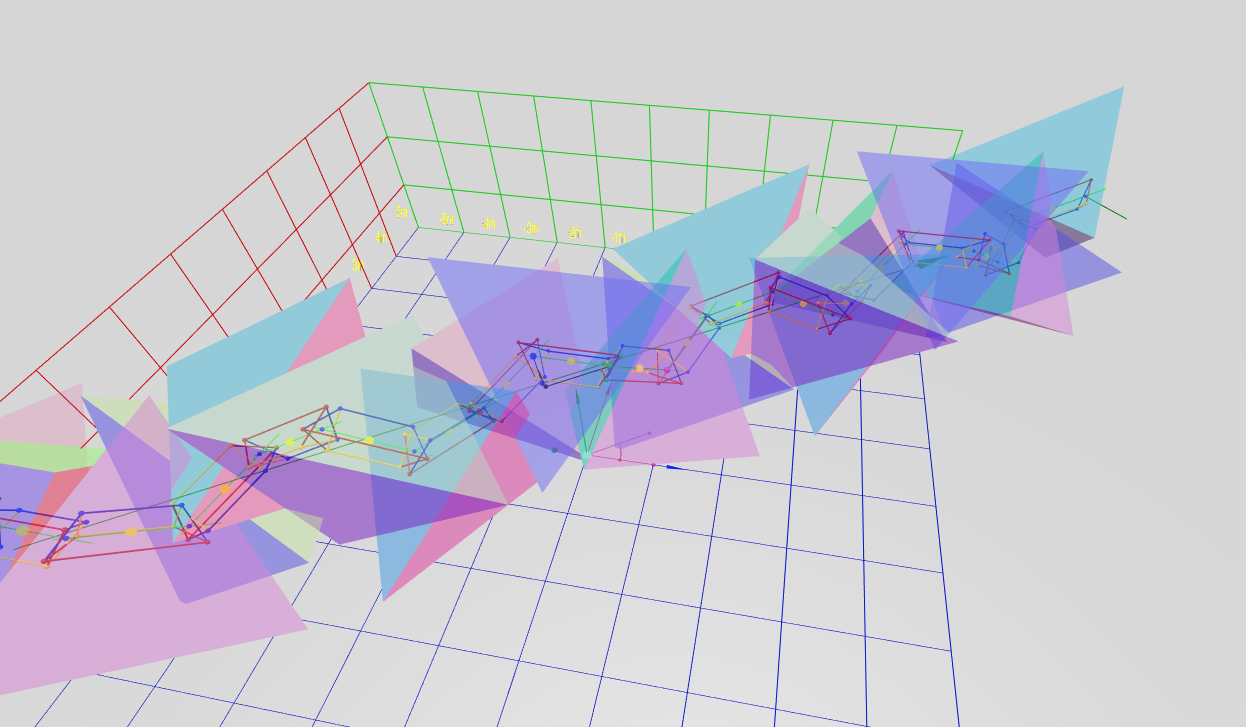
\includegraphics[width=0.80\textwidth]{figures/Period7Tetrahelix.png}
     \caption{ A Period-7 Tetrahelix generated with a twist of 80.43\degree}
  \label{fig:periodseven}
\end{figure}

Such a tetrahelix will
of course differ to some extent by being more or less ``jagged'' compared to the
BC helix. This related paper\cite{sadler2019periodic} has produced an analytic
formula specifically related to the tetrahedron. Presumably the interactive
software described here would assist in the search for analytic descriptions
of other {\em Platonic Helices}, or would allow an appoximation
to discovered quickly and simply visually.


\section{The Platonic Helices}

\label{sec:platonic}

In order to demonstrate the utility of the calculations explained in this paper,
periodic chains of the five regular Platonic solids joined face-to-face so that their vertices coincide,
which form {\em Platonic helices}, are explored.
Such tetrahelices, icosahelices, octahelices and dodecahelices
have been mentioned in a number of papers\cite{elgersma2016quadrahelix,elgersma2017asymptotically,babiker2012combinatorial,lord2001sphere}, but not exhaustively studied in
the purely helical form.
We propose the name {\em cubahelix} for the helix made from cubes, as opposed to the equivalent
but cumbersome {\em hexahedronahelix}.
Because in some cases Platonic segmented helices may be found in nature or
related to structures found in nature\cite{lord2004gamma,pearce1990structure},
it would be convenient to have a table, and images, of all such Platonic segmented helices for reference.

To construct a specific periodic chain from a Platonic solid,
one must decide which faces are joined by the rule.
Additionally, one must determine a twist
$\tau$ as part of the rule, and this twist must be chosen from a small set if the vertices are to coincide.
The set of vertex-matching twists differs slightly depending on the face chosen for octahedron, dodecahedron, and icosahedron
(but not for the tetrahedron and the cube). The number of twists in a set will always be equal to the number of sides on a face.

Therefore the number of Platonic helices is in principle a summation of a number of faces times a number of sides, or
$4 \cdot 3 + 6 \cdot 4 + 8 \cdot 3 + 12 \cdot 5 + 20 \cdot 3 = 12 + 24 + 24 + 60 + 60 = 180$.
However, many of the possible helices will be indistinguishable if only the shapes produced are considered,
as opposed to considering completely labeled or colored faces.
Furthermore, every non-toroidal helix will come in a clockwise and anti-clockwise version.
However, it is sensible to disallow rules such as ``attach face zero to face zero''
which would constitute
``doubling back''\cite{elgersma2016quadrahelix,elgersma2017asymptotically}.
The transformation matrix for such a rule would be the identity matrix.
It produces an object axis of zero length, a radius of zero, and
a travel of zero. It produces perfect self-intersection---the entire
degenerate helix would appear to be a simply a single Platonic solid.

Using the math in this paper and a computer, it is easy to evaluate all 180 helices,
place them in a table (see Table \ref{table:platonic}), and group them
by radius and travel (collapsing chirality).
The result is 28 unique shapes. In this number, no provision was made to exclude
self-intersection,
which does occur, but might not matter to
an aerospace engineer building a collapsible space frame of rods and joints.
In the language of Elgersma and Wagon\cite{elgersma2016quadrahelix,elgersma2017asymptotically}, not
all of the 28 Platonic helices are {\em embedded}.

With those caveats, the helices in Table \ref{table:platonic}, exemplified by
accompanying figures and renderable
interactively on the calculator page, represent an exhaustive catalog,
colloquially called a ``zoo'', of all Platonic helices.

In Table \ref{table:platonic}, column {\em C-Face} refers to the
face as numbered by the THREE.js software\cite{dirksen2013learning},
which is somewhat arbitrary. The {\em \# Analogs}
column gives the number of Platonic Helices with the same shape, or the enantiomer of it,
that is, the same
shape in either the clockwise or anti-clockwise direction.
This list can be expanded completely on our interactive website.

Clearly, for each solid there is a change in twist which keeps the vertices on
two joined faces coincident and
aligned if they start aligned. This is $2\pi/n$,
where $n$ is the number of sides in a face. The base twist that creates
a perfect face-to-face match depends not only on the solid but the face conjoined to.
For each of the Platonic
solids, the base angle was found by visual inspection and trial and error.
The twist $\tau$ of a species
of helix is given in the column below.

\begin{table}[ht]
\caption{The Platonic Helices} % title of Table
\centering % used for centering table
\begin{tabular}{l l r r r r r r r}
  \hline\hline %inserts double horizontal lines
  Name & Solid & \# Analogs & C-Face \# & $ \tau $ & radius & $ \theta $ & d & $ \phi $ \\ [0.5ex] % inserts table
%heading
  \hline % inserts single horizontal line
Tetrahelix & Tet &	6 &	1 &	-120 &	0.094 &	131.810	& -0.516 & 161.565 \\
Tetratorus & Tet & 	3 &	1 &	0    &	0.471 &	70.529	& 0.000	& 90.000 \\
\hline %inserts single line
Boxbeam & Cub &	4 &	1 &	-180 &	0.000 &	0.000 &	1.000 &	0.000 \\
Staircase & Cub &	4 & 	2 &	-180 &	0.000 &	0.000 &	0.707 &	0.000 \\
Blockhelix & Cub & 	8 & 	2 & 	-90  &	0.236 &	120.000 & -0.577 & 144.736 \\
Cubatorus & Cub &	4 &	2 &	0 &	0.500 &	90.000 & 0.000 & 90.000 \\
\hline %inserts single line
Octabeam & Oct &	3 &	5 &	-60 &	0.000 &	0.000 &	1.155 &	0.000 \\
Octaspiky & Oct &	6 &	1 &	-120 &	0.148 &	146.443 & -0.603 & 154.761 \\
Octamedium & Oct &	6 &	2 &	-120 &	0.163 &	131.810 & -0.894 & 161.565 \\
Octagear & Oct &	3 &	1 &	0 &	0.408 &	109.471 & 0.000	& 90.000 \\
Treestar & Oct &	3 &	2 &	0 &	0.816 &	70.529 & 0.000 & 90.000 \\
\hline %inserts single line
Dodecabeam & Dod &	5 &	8 &	-108 &	0.000 &	0.000 &	1.589 &	0.000 \\
Dodecadoubler & Dod &	10 &	1 &	-144 &	0.113 &	161.301 &-0.805 & 164.550 \\
The Alternater & Dod &	10 &	2 &	-144 &	0.118 &	149.520 &-1.333	& 170.306 \\
Dodecashaft & Dod &	10 &	1 &	-72 &	0.351 &	129.657	&-0.543 & 130.501 \\
Dodecagear & Dod &	5 &	1 &	0 &	0.491 &	116.565	& 0.000	& 90.000 \\
Dodecacorkscrew & Dod &	10 &	2 &	-72 &	0.546 &	93.026 & -1.095 & 144.110 \\
Dodecadonut & Dod &	5 &	2 &	0 &	1.286 &	63.435 & 0.000 & 90.000 \\
\hline %inserts single line
Pearlshaft & Ico &	3 &	13 &	-60 &	0.000 &	0.000 &	1.589 & 0.000 \\
Quasi-planar & Ico &	6 &	8 &	165 &	0.049 &	167.764 & 1.294 & 4.347 \\
Two Strands & Ico &	6 &	1 &	120 &	0.137 &	159.446	& 0.499 & 28.340 \\
Slow Twist & Ico &	6 &	12 &	120 &	0.169 &	124.309	& 1.454	& 11.641 \\
Rock Candy & Ico &	12 &	2 &	120 &	0.204 &	146.443	& 0.830 & 25.239 \\
Icosa Tree Star & Ico &	3 &	1 &	0 &	0.304 &	138.190	& 0.000	& 90.000 \\
Icosacorkscrew & Ico &	6 &	8 &	-75 &	0.512 &	99.253	& -1.037 & 143.042 \\
Planar point cluster & Ico &	6 &	2 &	0 &	0.562 &	109.471 & 0.000 & 90.000 \\
Big Icosacorkscrew  & Ico &	6 &	8 &	45 &	0.803 &	82.064 & 0.756 & 54.343 \\
The Wheel & Ico &	3 &	12 &	0 &	2.080 &	41.810 & 0.000 & 90.000 \\
\hline %inserts single line
\end{tabular}
\label{table:platonic} % is used to refer this table in the text
\end{table}

\subsection{Qualitative Descriptions and Interesting Shapes}

For fun and to facilitate conversation, we have given all
28 of these Platonic helices descriptive nicknames.
%% \footnote{These impressions
%%   are likely to be incomprehensible to a non-native speaker of English, or even to
%%   someone not born in America in the 1960's. We apologize for this, and hope the value of connoting the shape outweighs this cultural bias.}.
A few of these are interesting enough
to be worthy of particular mention, and comparing them
shows the possibility of designing structures using nothing but Platonic solids.
The math in this paper works equally well with irregular shapes as well,
allowing continuous spectra of designed structures from repeated shapes
or molecules.

\begin{itemize}
\item The ``Blockhelix'' (Figure \ref{fig:blockhelix}) is a cubic rectilinear structure in which all angles are right angles; nonetheless
  a segmented helix hides inside it which is perhaps not apparent to the human eye at first glance.
\begin{figure}
     \centering
     \includegraphics[width=0.40\textwidth]{figures/Blockhelix.png}
     \caption{The Blockhelix}
  \label{fig:blockhelix}
\end{figure}

\item The ``Pearlshaft'' (Figure \ref{fig:pearlshaft}). Conjoining parallel faces always produces a {\em shaft}. This icosahedron, being relatively round,
  resembles a string of pearls.
\begin{figure}
     \centering
     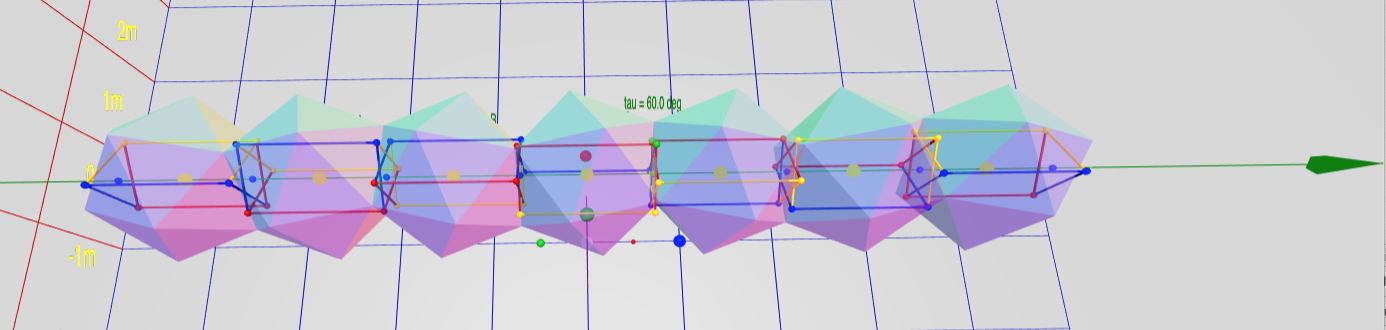
\includegraphics[width=0.40\textwidth]{figures/PearlShaft.png}
     \caption{The Pearlshaft}
  \label{fig:pearlshaft}
\end{figure}

\item However, shaft-like helices exist which do not join opposite faces. The ``Dodecashaft'' (Figure \ref{fig:dodecashaft}) is a remarkably tight
  non-self-intersecting dodecahelix with very narrow gaps between objects.
  Such a configuration
  might be formed by nanofibers under pressure.
\begin{figure}
     \centering
     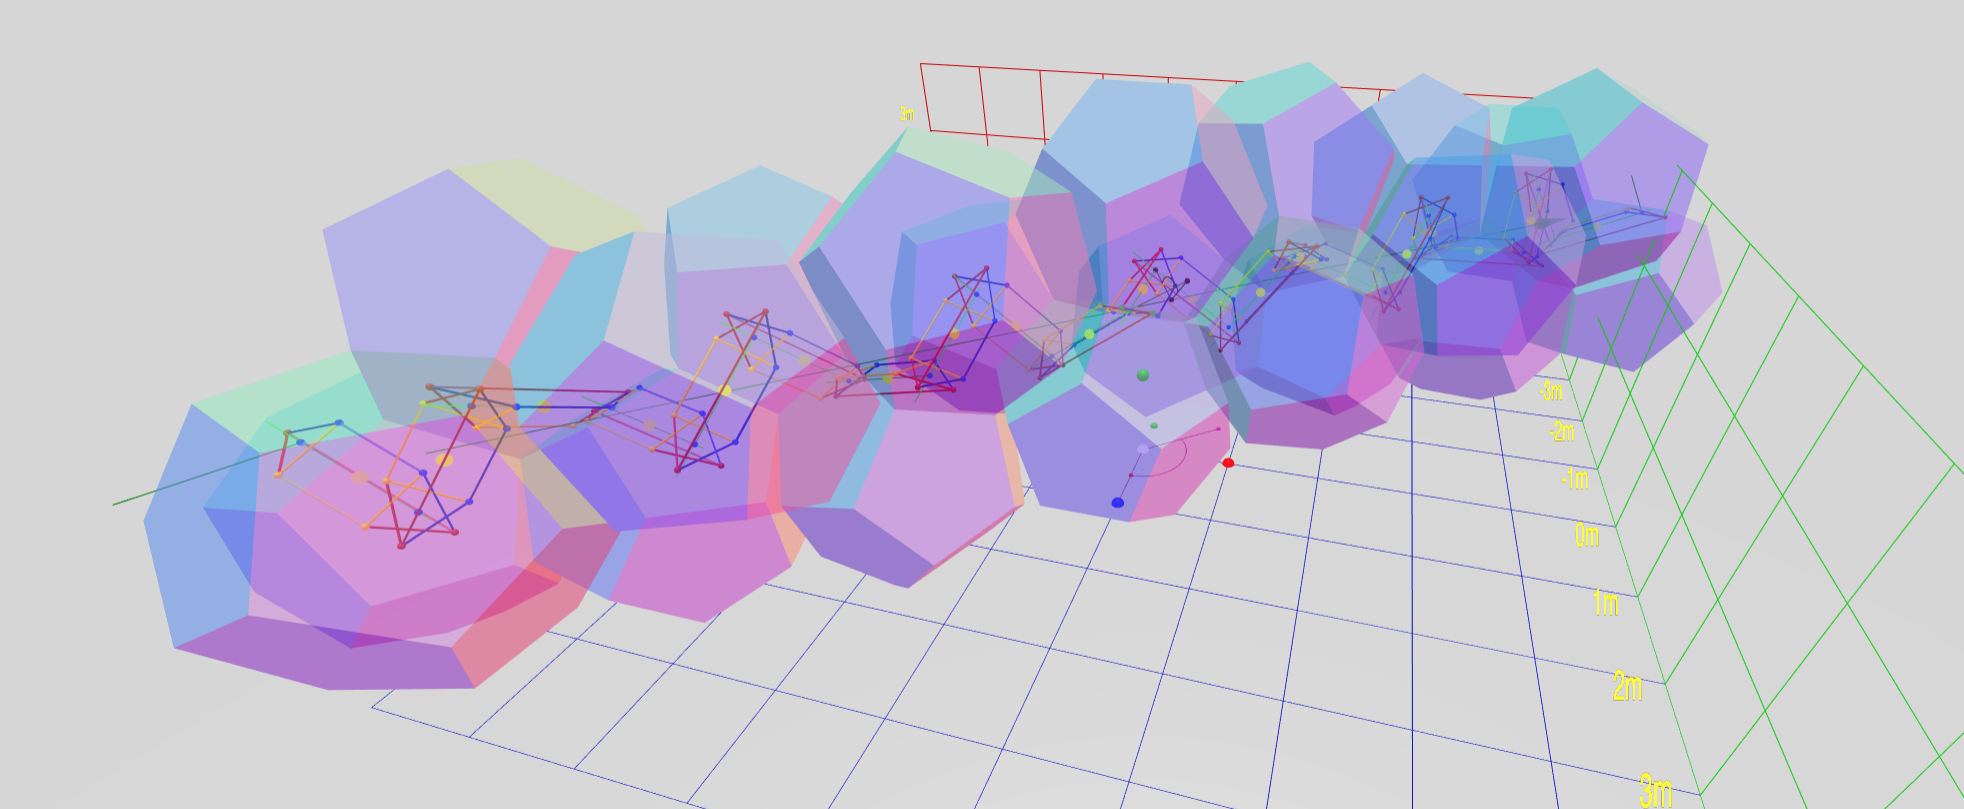
\includegraphics[width=0.40\textwidth]{figures/Dodecashaft.png}
     \caption{The Dodecashaft}
  \label{fig:dodecashaft}
\end{figure}
\item The ``Dodecadoubler'' (Figure \ref{fig:dodecadoubler}) presents the appearance of being a double helix, even though in fact it is a single helix with
  a simple twist of 72 $\degree$ from the ``Dodecashaft''.
\begin{figure}
     \centering
     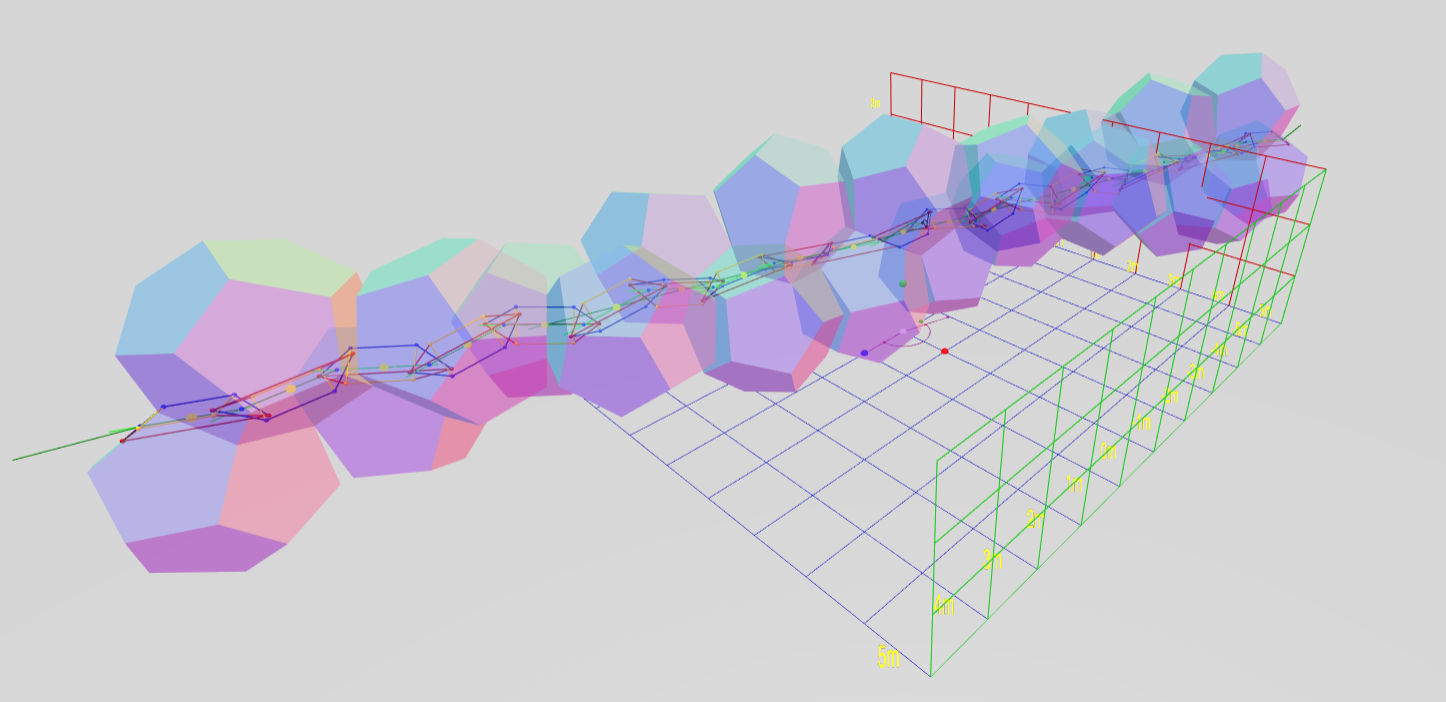
\includegraphics[width=0.40\textwidth]{figures/Dodecadoubler.png}
     \caption{The Dodecadoubler}
  \label{fig:dodecadoubler}
\end{figure}
\item The ``Dodecacorkscrew'' (Figure \ref{fig:dodecacorkscrew}) is a contrasting example of a loose helix, reminiscent of a corkscrew for opening wine bottles.
\begin{figure}
     \centering
     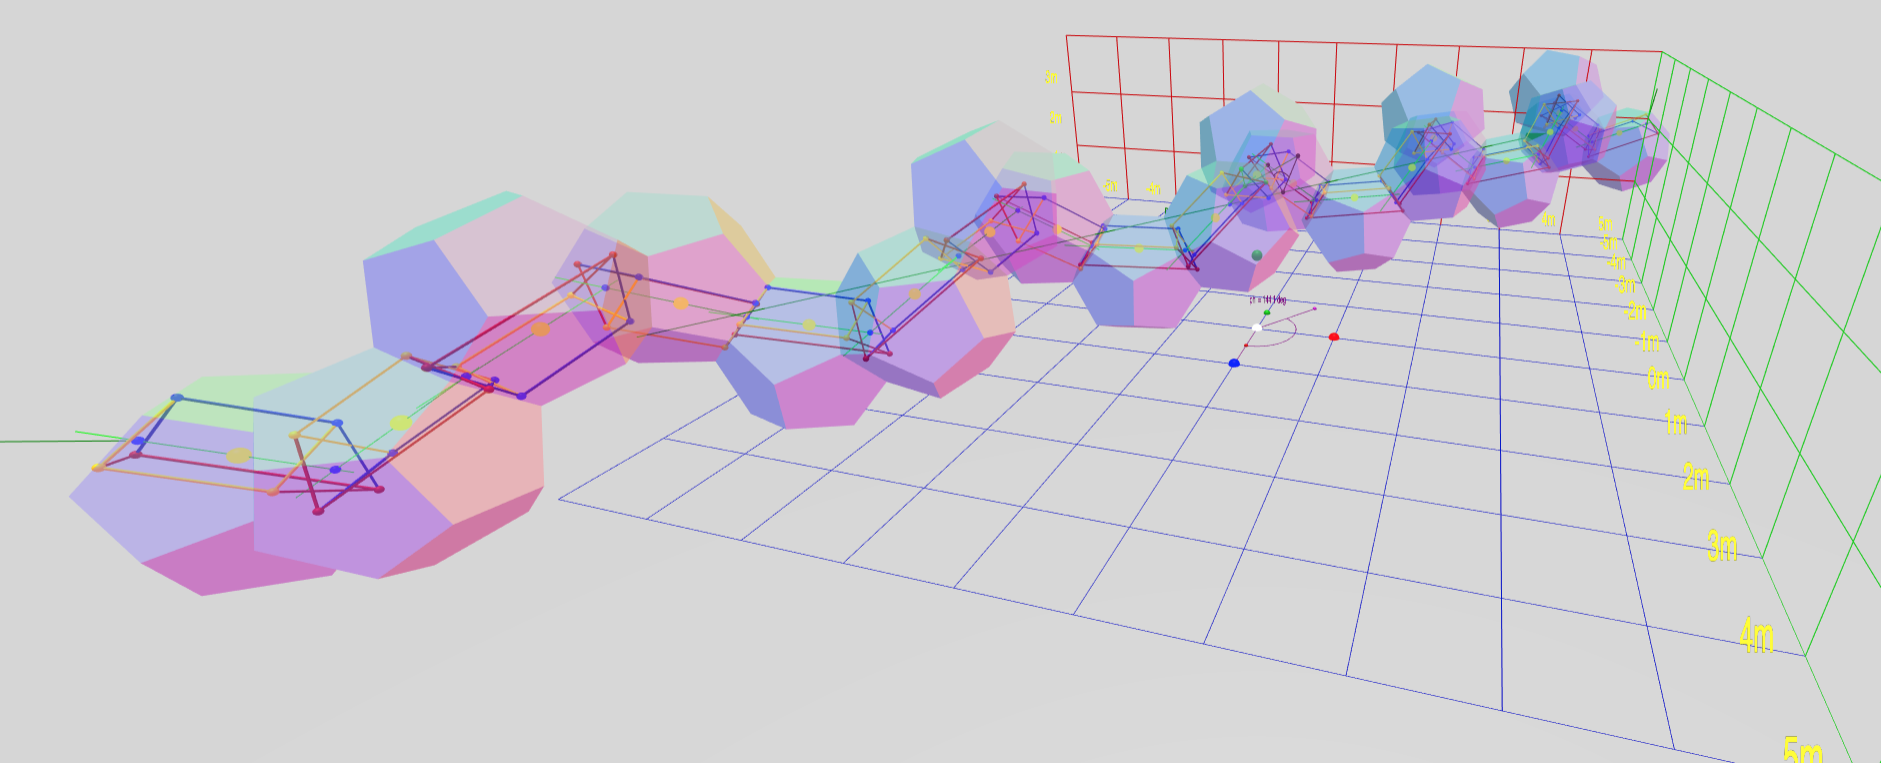
\includegraphics[width=0.40\textwidth]{figures/Dodecacorkscrew.png}
     \caption{The Dodecacorkscrew}
  \label{fig:dodecacorkscrew}
\end{figure}
\item The ``Quasi-planar'' (Figure \ref{fig:quasiplanar}) icosahelix presents a slowly twisting metahelix, so perhaps 10 icosahedron could be said to ``lay flat''. If this were
  a molecule or a physical structure made of less-than-perfectly rigid members, it might be possible to force it into a pure planar configuration,
  thus wrapping a cylinder or a plane, studding it with icosahedra.
\begin{figure}
     \centering
     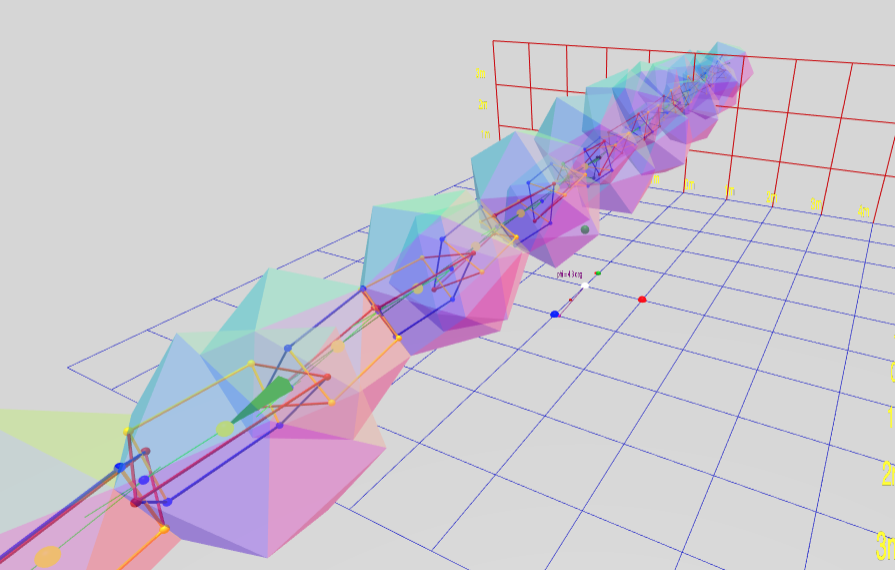
\includegraphics[width=0.40\textwidth]{figures/Planar.png}
     \caption{Quasi-planar icosahelix}
  \label{fig:quasiplanar}
\end{figure}
\item ``Two Strands'' (Figure \ref{fig:twostrands}) is similar to the ``Dodecadoubler'' but even more
  visually striking. It is reminiscent of a depiction of a DNA double
  helix.
\begin{figure}
     \centering
     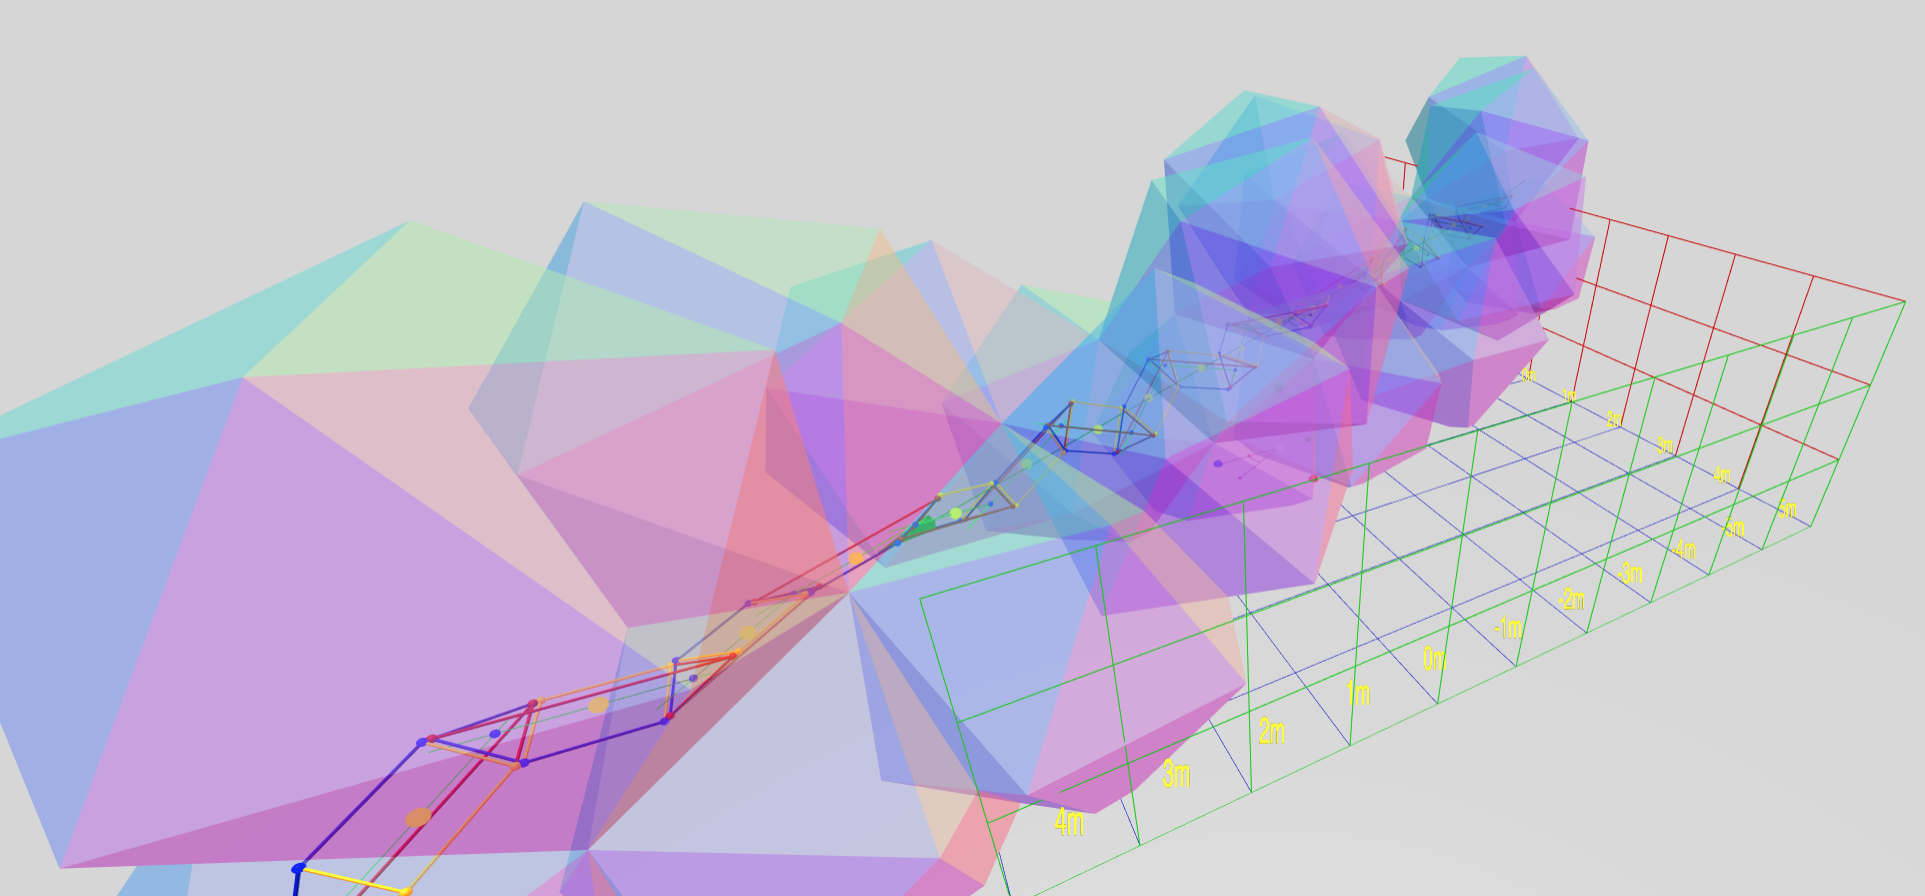
\includegraphics[width=0.40\textwidth]{figures/TwoStrands.png}
     \caption{Two Strands}
  \label{fig:twostrands}
\end{figure}
\item The ``Wheel'' (Figure \ref{fig:thewheel}) resembles a modern car tire
  in proportions.
  All Platonic solids and indeed all shapes have torus-like
  configurations. In general they do not ``close'' perfectly. There is a gap that prevents the final faces from fitting together perfectly.
  However, a tiny adjustment could be made to the repeated shape to close this gap.
\begin{figure}
     \centering
     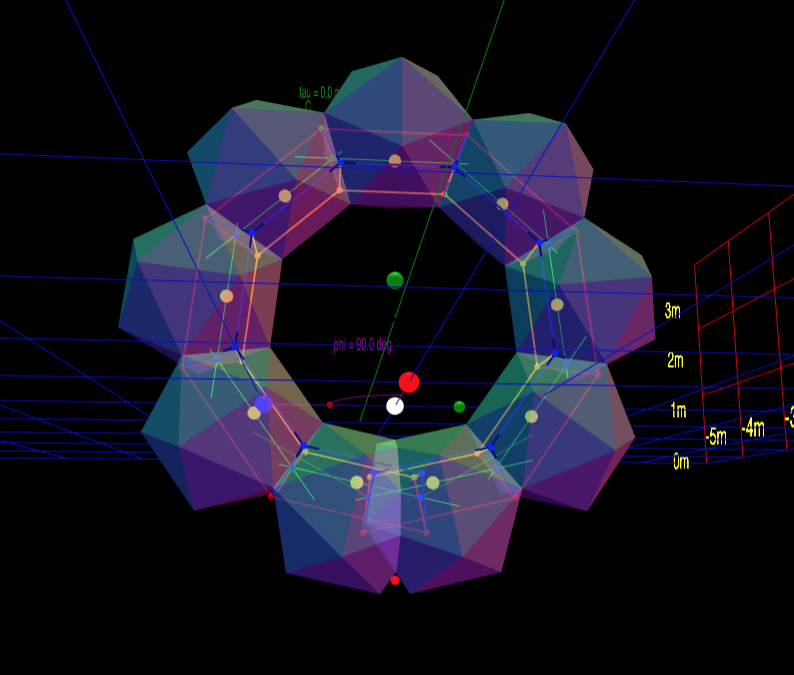
\includegraphics[width=0.40\textwidth]{figures/TheWheel.png}
     \caption{The Wheel}
  \label{fig:thewheel}
\end{figure}
\end{itemize}

\section{Future Work}

The algorithms and software described herein allow numerical calculation of the intrinsic properties of these
Platonic helices, but it would be even better to describe them
with closed-form expressions,
as Coxeter did for the Boerdijk-Coxeter tetrahelix.
The math and the algorithms are simple enough that if coded in a symbolic algebra system,
or with careful work, closed-form
expressions could be produced for all the regular Platonic helices.
These would be interesting if they happen to be short; there is no reason to
believe they will be. The same work could be done for the Archimedean solids. The current work would
serve as a useful validation check and intuition-builder for such work.

There may exist a closed-form expression for twist $\tau$ which produces a desired helix angle $\psi$.
The website implements
an iterative algorithm to find it, which is practical but less elegant.

\section{Acknowledgements}

Thanks to Prof. Eric Lord for his direct communication.
The enthusiasm of the participants of the 2018 Public Invention Mathathon
initiated this work.

\begin{adjustwidth}{-\extralength}{0cm}
\bibliographystyle{unsrt}
\bibliography{shelix}
\end{adjustwidth}


% If authors have biography, please use the format below
\section*{Short Biography of Authors}
\bio
{\raisebox{-0.35cm}{\includegraphics[width=3.5cm,height=5.3cm,clip,keepaspectratio]{Figures/author1.pdf}}}
{\textbf{Robert L. Read} This is a biography.}

\end{document}

\section{References that need to be studied or reviewed}


Note further that Equations 7 and 8 of this paper\cite{kahn1989defining} give BETTER equations for radius $r$ and the distance $d$ than what I have so far given. Note: I've studied this; I'm not sure there is anything worth doing there.

This is a discussion of segmented coils in a protein structure:

\url{https://www.sciencedirect.com/science/article/pii/0022283688903701}

A modern helix structure protein paper:

\url{https://www.sciencedirect.com/science/article/pii/S1476927108000583}


``Simulation of Suspensions of Helical Rigid Fibers'' Y Al-Hassan : British Journal of Mathematics and Computer Science
(PDF downloaded)

``HELFIT: Helix fitting by a total least squares method'' : This needs to be studied closely!
\url{https://www.sciencedirect.com/science/article/pii/S1476927108000418}

QHELIX: A Computational Tool for the Improved Measurement of Inter-Helical Angles in Proteins
\url{https://link.springer.com/article/10.1007/s10930-007-9097-9}

Note:''On the Screw Axes and Other Special Lines Associated With Spatial Displacements of a Rigid Body''
\url{http://manufacturingscience.asmedigitalcollection.asme.org/article.aspx?articleid=1439697}

Note: An historical review of the theoretical development of rigid body displacements from Rodrigues parameters to the finite twist
\url{https://www.sciencedirect.com/science/article/pii/S0094114X0500087X}


\section{References Reviewed but not worth citing}

This is a long, expensive book, but it is not relevant relevant\cite{hyde1996language}:
\url{https://books.google.com/books?hl=en&lr=&id=1LZlSZ7ORrQC&oi=fnd&pg=PP1&ots=0hSEwJvlUB&sig=xNG9UWv_H1OXHwaOiOBJN7TW6xA#v=onepage&q&f=false}


Note: There is another long, deep book that needs to be obtained and studied\cite{sadoc2006geometrical}.
\url{https://books.google.com/books?hl=en&lr=&id=FHPlDWvz1bEC&oi=fnd&pg=PP1&ots=TsOnodavEZ&sig=HO86UUVlqRVWGqY-Tv02nb7x7NA#v=onepage&q&f=false}


This talks about tuning the period of a helix inside a nanopore:

\url{https://aip.scitation.org/doi/abs/10.1063/1.4794785}



\url{https://www.researchgate.net/publication/236066626_Segmented_helical_structures_formed_by_ABC_star_copolymers_in_nanopores}


``Local Frustration Determines Molecular and Macroscopic Helix Structures''

\url{https://pubs.acs.org/doi/abs/10.1021/jp4040503}


NOTE: This is a discussion of representing joint angles, it is not obvious how valuable it is:
\url{https://www.clinbiomech.com/article/S0268-0033(98)00080-1/abstract}

\url{https://www.win.tue.nl/~wstomv/publications/mathmitering-final.pdf}


\url{https://gist.github.com/peteristhegreat/3b76d5169d7b9fc1e333}

\url{https://www.sciencedirect.com/science/article/pii/S0022309307005583}



This may be worth reading:
\url{https://link.springer.com/article/10.1007/PL00011063}

Some discussion of ``screw transformations''
\url{http://dergipark.gov.tr/download/article-file/56483}

``Analyzing Protein Structure Using Almost Delaunay Tetrahedra''

\url{https://www.researchgate.net/profile/Alexander_Tropsha/publication/250901525_Analyzing_Protein_Structure_Using_Almost-Delaunay_Tetrahedra/links/5578584408ae75215870347c/Analyzing-Protein-Structure-Using-Almost-Delaunay-Tetrahedra.pdf}



\begin{figure}
     \centering
     
\includegraphics[width=0.80\textwidth]{figures/RotatingPlane.png}
     \caption{Planes Rotating About the $z$-axis}
  \label{fig:rotatingplane}
\end{figure}


\section{ To Do}

\begin{itemize}
\item finish proofread
\item Decide if that algorithm takes A or D as input
  \item Figure out if Joint Face Normal method is properly introduced, along with twist and other concepts
  \item Add chord, L, etc. to diagram.
  \item MAJOR BUG: C.z < 0 and B.z < 0 causes mismatch
\item Consider application here: https://imbicorg.blogspot.com/p/the-main-objective-of-conference-is-to.html
  \item Here: http://www.ramsaconference.com/
  \item Modify that so that it truly respects $\psi$ as an input.
\item Provide explanation, graphically, if need be, for
  the computation of $B_{ax}, B_{ay}, B_{az}$ in the general cases.
\item Clean up the code. 3 days
\item Go through each reference 1 day
\item Try to get list of references to the computation of a screw from an arbitrary matrix, and compare and contrast to our code. 1 day
\item Need to understand possibility of further simplifying specification of object.

\item Need to get this paper, by hook or by crook, and probably cite:
  Note: An historical review of the theoretical development of rigid body displacements from Rodrigues parameters to the finite twist
  \url{https://www.sciencedirect.com/science/article/pii/S0094114X0500087X}
    \item Bibliographic references do not appear to be as detailed as they should be.
  \end{itemize}
s
